% Options for packages loaded elsewhere
\PassOptionsToPackage{unicode}{hyperref}
\PassOptionsToPackage{hyphens}{url}
\PassOptionsToPackage{dvipsnames,svgnames,x11names}{xcolor}
%
\documentclass[
  letterpaper,
  DIV=11,
  numbers=noendperiod]{scrartcl}

\usepackage{amsmath,amssymb}
\usepackage{setspace}
\usepackage{iftex}
\ifPDFTeX
  \usepackage[T1]{fontenc}
  \usepackage[utf8]{inputenc}
  \usepackage{textcomp} % provide euro and other symbols
\else % if luatex or xetex
  \usepackage{unicode-math}
  \defaultfontfeatures{Scale=MatchLowercase}
  \defaultfontfeatures[\rmfamily]{Ligatures=TeX,Scale=1}
\fi
\usepackage{lmodern}
\ifPDFTeX\else  
    % xetex/luatex font selection
\fi
% Use upquote if available, for straight quotes in verbatim environments
\IfFileExists{upquote.sty}{\usepackage{upquote}}{}
\IfFileExists{microtype.sty}{% use microtype if available
  \usepackage[]{microtype}
  \UseMicrotypeSet[protrusion]{basicmath} % disable protrusion for tt fonts
}{}
\makeatletter
\@ifundefined{KOMAClassName}{% if non-KOMA class
  \IfFileExists{parskip.sty}{%
    \usepackage{parskip}
  }{% else
    \setlength{\parindent}{0pt}
    \setlength{\parskip}{6pt plus 2pt minus 1pt}}
}{% if KOMA class
  \KOMAoptions{parskip=half}}
\makeatother
\usepackage{xcolor}
\usepackage[top=1in,bottom=1in,left=1.5in,right=1in]{geometry}
\setlength{\emergencystretch}{3em} % prevent overfull lines
\setcounter{secnumdepth}{-\maxdimen} % remove section numbering
% Make \paragraph and \subparagraph free-standing
\makeatletter
\ifx\paragraph\undefined\else
  \let\oldparagraph\paragraph
  \renewcommand{\paragraph}{
    \@ifstar
      \xxxParagraphStar
      \xxxParagraphNoStar
  }
  \newcommand{\xxxParagraphStar}[1]{\oldparagraph*{#1}\mbox{}}
  \newcommand{\xxxParagraphNoStar}[1]{\oldparagraph{#1}\mbox{}}
\fi
\ifx\subparagraph\undefined\else
  \let\oldsubparagraph\subparagraph
  \renewcommand{\subparagraph}{
    \@ifstar
      \xxxSubParagraphStar
      \xxxSubParagraphNoStar
  }
  \newcommand{\xxxSubParagraphStar}[1]{\oldsubparagraph*{#1}\mbox{}}
  \newcommand{\xxxSubParagraphNoStar}[1]{\oldsubparagraph{#1}\mbox{}}
\fi
\makeatother


\providecommand{\tightlist}{%
  \setlength{\itemsep}{0pt}\setlength{\parskip}{0pt}}\usepackage{longtable,booktabs,array}
\usepackage{calc} % for calculating minipage widths
% Correct order of tables after \paragraph or \subparagraph
\usepackage{etoolbox}
\makeatletter
\patchcmd\longtable{\par}{\if@noskipsec\mbox{}\fi\par}{}{}
\makeatother
% Allow footnotes in longtable head/foot
\IfFileExists{footnotehyper.sty}{\usepackage{footnotehyper}}{\usepackage{footnote}}
\makesavenoteenv{longtable}
\usepackage{graphicx}
\makeatletter
\def\maxwidth{\ifdim\Gin@nat@width>\linewidth\linewidth\else\Gin@nat@width\fi}
\def\maxheight{\ifdim\Gin@nat@height>\textheight\textheight\else\Gin@nat@height\fi}
\makeatother
% Scale images if necessary, so that they will not overflow the page
% margins by default, and it is still possible to overwrite the defaults
% using explicit options in \includegraphics[width, height, ...]{}
\setkeys{Gin}{width=\maxwidth,height=\maxheight,keepaspectratio}
% Set default figure placement to htbp
\makeatletter
\def\fps@figure{htbp}
\makeatother
% definitions for citeproc citations
\NewDocumentCommand\citeproctext{}{}
\NewDocumentCommand\citeproc{mm}{%
  \begingroup\def\citeproctext{#2}\cite{#1}\endgroup}
\makeatletter
 % allow citations to break across lines
 \let\@cite@ofmt\@firstofone
 % avoid brackets around text for \cite:
 \def\@biblabel#1{}
 \def\@cite#1#2{{#1\if@tempswa , #2\fi}}
\makeatother
\newlength{\cslhangindent}
\setlength{\cslhangindent}{1.5em}
\newlength{\csllabelwidth}
\setlength{\csllabelwidth}{3em}
\newenvironment{CSLReferences}[2] % #1 hanging-indent, #2 entry-spacing
 {\begin{list}{}{%
  \setlength{\itemindent}{0pt}
  \setlength{\leftmargin}{0pt}
  \setlength{\parsep}{0pt}
  % turn on hanging indent if param 1 is 1
  \ifodd #1
   \setlength{\leftmargin}{\cslhangindent}
   \setlength{\itemindent}{-1\cslhangindent}
  \fi
  % set entry spacing
  \setlength{\itemsep}{#2\baselineskip}}}
 {\end{list}}
\usepackage{calc}
\newcommand{\CSLBlock}[1]{\hfill\break\parbox[t]{\linewidth}{\strut\ignorespaces#1\strut}}
\newcommand{\CSLLeftMargin}[1]{\parbox[t]{\csllabelwidth}{\strut#1\strut}}
\newcommand{\CSLRightInline}[1]{\parbox[t]{\linewidth - \csllabelwidth}{\strut#1\strut}}
\newcommand{\CSLIndent}[1]{\hspace{\cslhangindent}#1}

\usepackage{booktabs}
\usepackage{longtable}
\usepackage{array}
\usepackage{multirow}
\usepackage{wrapfig}
\usepackage{float}
\usepackage{colortbl}
\usepackage{pdflscape}
\usepackage{tabu}
\usepackage{threeparttable}
\usepackage{threeparttablex}
\usepackage[normalem]{ulem}
\usepackage{makecell}
\usepackage{xcolor}
\usepackage{lineno}\linenumbers
\KOMAoption{captions}{tableheading}
\makeatletter
\@ifpackageloaded{tcolorbox}{}{\usepackage[skins,breakable]{tcolorbox}}
\@ifpackageloaded{fontawesome5}{}{\usepackage{fontawesome5}}
\definecolor{quarto-callout-color}{HTML}{909090}
\definecolor{quarto-callout-note-color}{HTML}{0758E5}
\definecolor{quarto-callout-important-color}{HTML}{CC1914}
\definecolor{quarto-callout-warning-color}{HTML}{EB9113}
\definecolor{quarto-callout-tip-color}{HTML}{00A047}
\definecolor{quarto-callout-caution-color}{HTML}{FC5300}
\definecolor{quarto-callout-color-frame}{HTML}{acacac}
\definecolor{quarto-callout-note-color-frame}{HTML}{4582ec}
\definecolor{quarto-callout-important-color-frame}{HTML}{d9534f}
\definecolor{quarto-callout-warning-color-frame}{HTML}{f0ad4e}
\definecolor{quarto-callout-tip-color-frame}{HTML}{02b875}
\definecolor{quarto-callout-caution-color-frame}{HTML}{fd7e14}
\makeatother
\makeatletter
\@ifpackageloaded{caption}{}{\usepackage{caption}}
\AtBeginDocument{%
\ifdefined\contentsname
  \renewcommand*\contentsname{Table of contents}
\else
  \newcommand\contentsname{Table of contents}
\fi
\ifdefined\listfigurename
  \renewcommand*\listfigurename{List of Figures}
\else
  \newcommand\listfigurename{List of Figures}
\fi
\ifdefined\listtablename
  \renewcommand*\listtablename{List of Tables}
\else
  \newcommand\listtablename{List of Tables}
\fi
\ifdefined\figurename
  \renewcommand*\figurename{Figure}
\else
  \newcommand\figurename{Figure}
\fi
\ifdefined\tablename
  \renewcommand*\tablename{Table}
\else
  \newcommand\tablename{Table}
\fi
}
\@ifpackageloaded{float}{}{\usepackage{float}}
\floatstyle{ruled}
\@ifundefined{c@chapter}{\newfloat{codelisting}{h}{lop}}{\newfloat{codelisting}{h}{lop}[chapter]}
\floatname{codelisting}{Listing}
\newcommand*\listoflistings{\listof{codelisting}{List of Listings}}
\makeatother
\makeatletter
\makeatother
\makeatletter
\@ifpackageloaded{caption}{}{\usepackage{caption}}
\@ifpackageloaded{subcaption}{}{\usepackage{subcaption}}
\makeatother

\ifLuaTeX
  \usepackage{selnolig}  % disable illegal ligatures
\fi
\usepackage{bookmark}

\IfFileExists{xurl.sty}{\usepackage{xurl}}{} % add URL line breaks if available
\urlstyle{same} % disable monospaced font for URLs
\hypersetup{
  pdftitle={Chapter 3},
  pdfauthor={Tyler Wiederich},
  colorlinks=true,
  linkcolor={blue},
  filecolor={Maroon},
  citecolor={Blue},
  urlcolor={Blue},
  pdfcreator={LaTeX via pandoc}}


\title{Chapter 3}
\author{Tyler Wiederich}
\date{March 22, 2026}

\begin{document}
\maketitle
\begin{abstract}
The display of 3-dimensional (3D) data is often limited by how it can be
rendered. These renderings are typically presented as charts on
2-dimensional (2D) computer screens using 2D or 3D chart styles.
However, computer renderings do not provide the level of interactivity
of 3D charts that we experience in a 3D world, something which can be
accomplished through the use of 3D printing. In this paper, we describe
a study to compare 2D and 3D heatmaps rendered digitally or via 3D
printing and assess the findings of 3D printed charts for the use of
displaying statistical information.
\end{abstract}


\setstretch{2}
\subsection{Introduction}\label{introduction}

In the 20th century, advancements in technology made data visualizations
increasingly more affordable and accessible to a broader population. The
primary change in formal data visualizations was from hand-drawn charts
to computer-rendered charts (Tukey 1965), yet other technological
advances have allowed for data visualizations to enter other mediums.
These include the ability to effectively use the 3-dimensional (3D)
world around us with the novel use of 3D-printed charts. This newer type
of visualization has gained a small amount of traction in recent years
as a method of producing tangible charts
(\textbf{stusakIfYourMind2016?}; \textbf{huExploringNewParadigms2015b?};
\textbf{huronMakingDataPhysical2023?})

At this time, there are few, if any, studies that evaluate 3D-printed
charts for the purpose of displaying statistical information. This may
in part be due to the cost of materials and rendering times as compared
to charts produced on a computer. A single chart can take up to a day to
print, limiting the ability to quickly produce visualizations. Given the
nature of 3-dimensional data, viewing a 3D realization of statistical
information in a 3D environment is a realistic scenario that could
increase the ability for information extraction.

3D-printed visualizations have shown mixed or promising results across
many disciplines. Katsioloudis and Jones (2018) showed no evidence of a
statistical difference in the method of 3D renderings when tasked with
drawing a cross-sectional of a dodecahedron. This demonstrated that
spatial awareness between computer-rendered and 3D-printed shapes is not
largely different among engineering students. The use of 3D-printed maps
for navigation for visually impaired persons showed positive feedback by
Holloway et al. (2019), increasing the accessibility of navigation. In
the clinical setting, 3D-printed anatomy structures were well accepted
along with VR-glasses and 3D computer renderings (Muff et al. 2022).
With the rise of 3D-printed visualizations in scientific fields, we turn
our attention to their use for statistical graphics.

\subsubsection{Literature Review}\label{literature-review}

An identical dataset across multiple chart types does not ensure that
the data is perceived in the same way (Cleveland and McGill 1984;
Hofmann et al. 2012; Vanderplas, Cook, and Hofmann 2020). One of the
main factors in this phenomenon is how data is encoded into the chart.
These encodings include, but are not limited to, placement along axes,
lengths, areas, volumes, and color scales. For example, bar charts and
pie charts are two common visualizations that have long since been the
topic of debate (Eells 1926; Croxton and Stryker 1927; Cleveland and
McGill 1984). In the case of bar charts and pie charts, encodings are
represented by lengths and angles, respectively. Inherently, the
comparison of different chart types is a comparison of encodings due to
the changes in how data is being displayed.

Cleveland and McGill (1984) noted that estimates involving numerical
accuracy may decrease when increasing dimensionality of the encoding,
although this was not formally tested in their experiments. Their
reasoning was due to Stevens' power law, a mathematical formulation of
how magnitudes are perceived given different stimuli sources (Stevens
and Stevens 1986). The general form of the law is \(\psi(I)=kI^\alpha\),
where \(I\) is the magnitude of a stimulus, \(\psi(I)\) is the perceived
magnitude, \(k\) is a proportionality constant from the unit of the
stimulus, and \(\alpha\) is the exponent from the type of stimuli used.
Studies have estimated that lengths are perceived without bias (i.e.,
\(\alpha=1\)), but areas and volumes tend to have skewed perceptions
(Cleveland and McGill 1984). This indicates that lower-dimensional
charts may perform better when readers are tasked with extracting
numerical estimates from the chart, although this has been a topic of
debate in the last several decades.

There are mixed results in regard to the use of 3D charts, mostly
attributing to the purpose of the third dimension. When the extra
dimension does not convey meaningful information, estimates of accuracy
decrease and solution times increase as compared to equivalent 2D charts
(Fisher, Dempsey, and Marousky 1997; Zacks et al. 1998; Fischer 2000).
The same increase in solution time is seen when the third dimension is
utilized for displaying data, but can sometimes produce better error
rates than 2D charts (Barfield and Robless 1989; Kraus et al. 2020).
Additionally, when given the option of 2D or 3D charts for extracting
numerical information, the 2D charts showed increased preference and
confidence than their 3D counterparts (Barfield and Robless 1989;
Fisher, Dempsey, and Marousky 1997). It is worth noting that all of
these studies use 2D or virtual reality renderings of 3D charts and not
physical 3D charts.

Formal studies involving true 3D charts are limited, and it is unclear
if they follow the framework of existing theories on data
visualizations. Unlike paper and computer-rendered charts, constructing
true 3D charts inherently contains many additional factors that could
affect perception, such as chart materials, natural lighting,
interactivity, and viewing distance. Some of these factors have already
been shown to have an effect on computer renderings (Tarr and Kriegman
2001; Wang et al. 2022).

We hypothesize that 3D charts in 3D environments will produce better
information extraction than their computer-rendered counterparts.
Specifically, we compare 3D-printed charts to digital 2D and 3D
renderings. We suspect that this difference will hold across multiple
data sets and different magnitudes of stimuli. In this paper, we
evaluate the accuracy of numerical estimations on true 3D charts by
conducting a factorial experiment that assessed chart types and ratios
of pairs of stimuli. We discuss the construction of the stimuli and how
we closely matched the charts to compare 2D, 3D-digital, and 3D-printed
renderings of heatmap data.

\subsection{Methods}\label{methods}

Our study was designed to evaluate and expand the literature on
numerical estimation of dimensionality for 3D charts. In our study, we
focused on 2D and 3D heatmaps, which we carefully constructed to ensure
that differences can be attributed to the dimensionality of the chart.
All of our data and methods are publicly available for open science and
reproducibility at \url{https://github.com/TWiedRW/ch3-heat3d}. In this
section, we discuss the process of designing our experiment and
participant recruitment.

\subsubsection{Stimuli}\label{stimuli}

We denote ``stimuli'' to represent the magnitude of our chosen values.
In a 3D Cartesian space, the X- and Y- axes represent the coordinates of
the stimuli, and the Z-axis represents the value for the stimuli. Each X
and Y coordinate is represented by a square tile with a 1:1 aspect
ratio. For a 2D space, the Z-axis is replaced by a color gradient scale.
All stimuli and remaining randomly generated values range between 0 and
100 units. In this experiment, \(X=1, 2, \dots,10\) and
\(Y=1, 2,\dots,10\).

The design of our experiment made use of the method of constant stimuli,
where comparisons between stimuli are with respect to a stimulus that
remains the same magnitude (Kingdom and Prins 2016, chap. 3). We set the
constant stimuli at 50 units. For stimuli between 50 and 100, we set the
maximum stimuli value at 90 and equally partitioned the ratios of
stimuli with the constant stimuli, \(\frac{50}{90}=0.556\) to
\(\frac{50}{50}=1.0\), resulting in 4 varying stimuli values where 50 is
the smallest value. The same ratios obtained with stimuli between 50 and
90 were used to create 4 stimuli varying between 0 and 50, where 50 is
the largest value. Additionally, we also included a stimulus pair where
both values are 50, resulting in nine total pairs of stimuli. All
stimuli values can be found in Figure~\ref{fig-stimuli-values}.

\begin{figure}

\centering{


\includegraphics{index_files/figure-pdf/fig-stimuli-values-1.pdf}

}

\caption{\label{fig-stimuli-values}Values for stimuli in the heatmap
experiment. All values are paired with the constant stimuli of 50 units,
creating nine pairs of stimuli.}

\end{figure}%

To generate non-stimuli random values, we used a mixture distribution of
random uniform noise and a mathematical function to populate our
coordinate grid. The mathematical functions are scaled between 0 and
100, \(g(Z)=100\cdot\frac{Z-\min(Z)}{\max(Z)-min(Z)}\). Two datasets
were created for the experiment. The first dataset, called set 1, used
the formula for the top half of a sphere that is centered within our X
and Y coordinate grid,
\(f_1(X,Y)=\sqrt{7^2-(X-\bar{X})^2-(Y-\bar{Y})^2}\), where \(\bar{X}\)
and \(\bar{Y}\) are the averages of the \(X\) and \(Y\) coordinate
ranges. The second dataset is calculated similarly using the formula for
the bottom half of a sphere,
\(f_2(X,Y)=\sqrt{7^2-(X-\bar{X})^2+(Y-\bar{Y})^2}\). Denoting \(Z\) as
the random values, \(U(0,100)\) as a random variable drawn from a
continuous uniform distribution between 0 and 100, and \(X,Y\) as
heatmap coordinates, our random heatmap data is calculated in
Equation~\ref{eq-random-z} with \(c=0.3\). An example of varying \(c\)
values is presented in Figure~\ref{fig-random-z}.

\begin{equation}\phantomsection\label{eq-random-z}{
Z=c\cdot U(0,100)+(1-c)\cdot g(f_i(X,Y))
}\end{equation}

\begin{figure}

\begin{minipage}{0.20\linewidth}

\centering{


\includegraphics{plots/z100.png}

}

\subcaption{\label{fig-z100}\(c=0\)}

\end{minipage}%
%
\begin{minipage}{0.20\linewidth}

\centering{

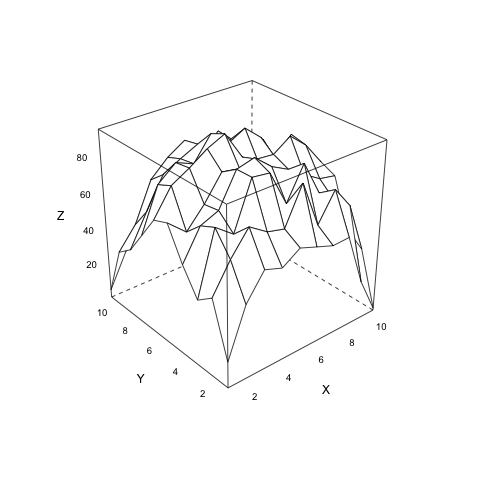
\includegraphics{plots/z75.png}

}

\subcaption{\label{fig-z75}\(c=0.25\)}

\end{minipage}%
%
\begin{minipage}{0.20\linewidth}

\centering{

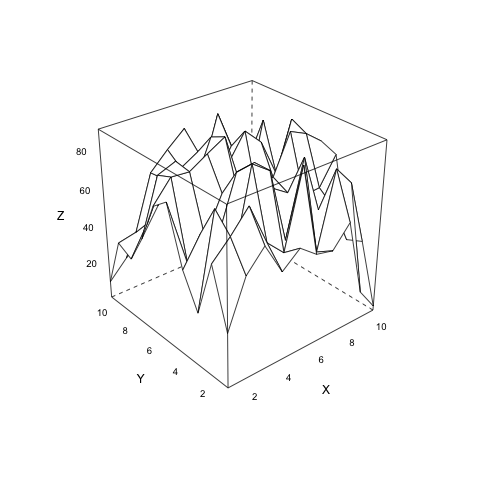
\includegraphics{plots/z50.png}

}

\subcaption{\label{fig-z50}\(c=0.5\)}

\end{minipage}%
%
\begin{minipage}{0.20\linewidth}

\centering{

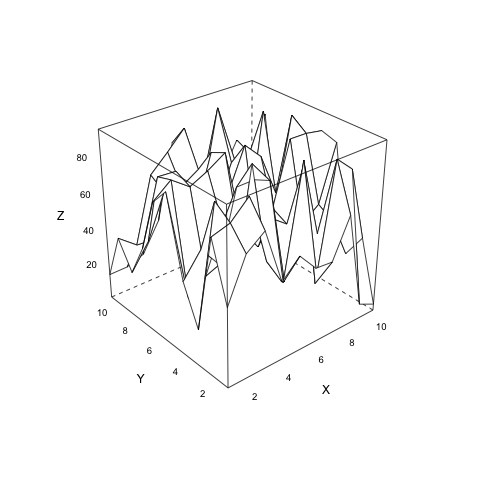
\includegraphics{plots/z25.png}

}

\subcaption{\label{fig-z25}\(c=0.75\)}

\end{minipage}%
%
\begin{minipage}{0.20\linewidth}

\centering{

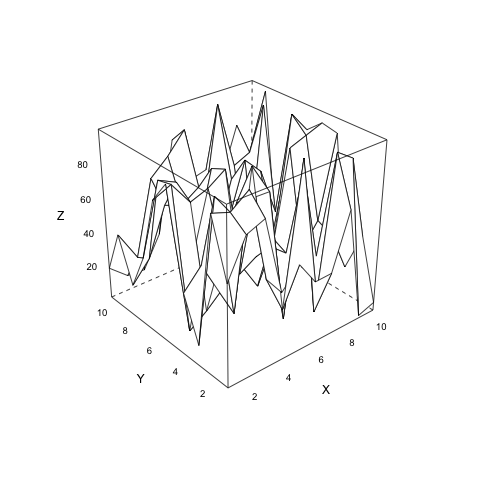
\includegraphics{plots/z0.png}

}

\subcaption{\label{fig-z0}\(c=1\)}

\end{minipage}%

\caption{\label{fig-random-z}Mixture distribution of
Equation~\ref{eq-random-z} using the formula for the top half of a
sphere. As \(c\) approaches 1, the distribution resembles uniform random
noise.}

\end{figure}%

The placement of stimuli values onto the randomly generated heatmap data
was done via simulation to try to make their placement look as natural
as possible. Twenty random heatmaps were generated. For each heatmap,
the non-constant stimuli was placed onto the coordinate such that the
difference between the stimuli and randomly generated value is
minimized. The constant stimuli was then placed onto a coordinate within
a Manhattan distance of three or four that minimizes the difference
between the constant stimuli and randomly generated values, where the
Manhattan distance is given by \(|X_i - X_j| + |Y_i - Y_j|\) for stimuli
\(i\) and \(j\). To ensure that stimuli placement is evenly positioned
across the heatmap, the count of stimuli was computed separately across
the X and Y axes. For example, in Data Set 1, the X-axis has four
stimuli in \(X=1\), three stimuli in \(X=2\), and so forth. Chi-squared
statistics were calculated for each axis and the heatmap with the
smallest average Chi-squared statistic was selected as the final
dataset. A visual inspection of this process showed that the stimuli
were not clustered in any one area of the chart and that the stimuli
look natural with respect to the random mixture distribution.

\begin{figure}

\begin{minipage}{0.50\linewidth}

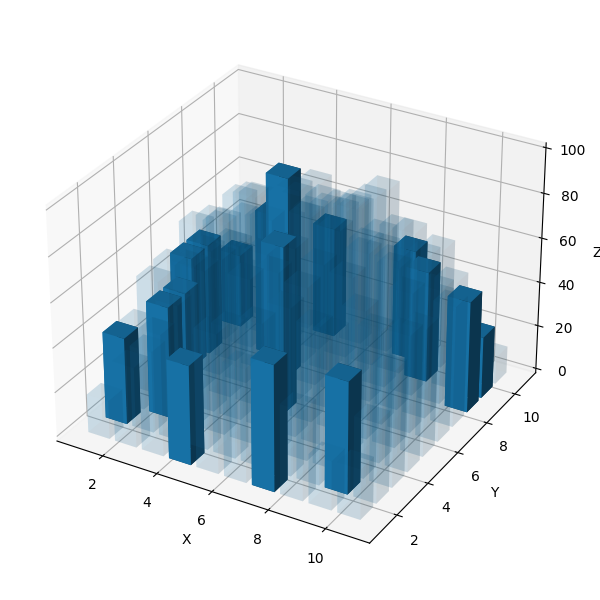
\includegraphics{../_images/stimuli-set1.png}

\subcaption{\label{}Placement of stimuli on Set 1}
\end{minipage}%
%
\begin{minipage}{0.50\linewidth}

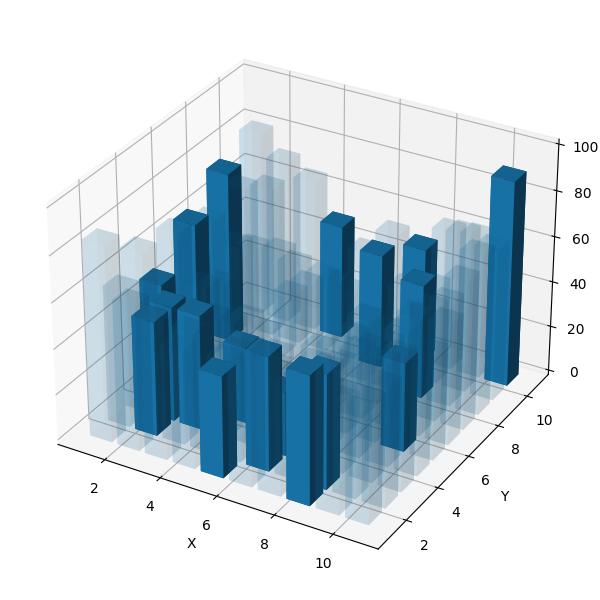
\includegraphics{../_images/stimuli-set2.png}

\subcaption{\label{}Placement of stimuli on Set 2}
\end{minipage}%

\caption{\label{fig-placement}Placement of stimuli on the two data sets.
Bars with solid fills are the fixed stimuli values, where opaque bars
are randomly generated.}

\end{figure}%

\subsubsection{Charts}\label{charts}

Three types of charts were considered for this study: 2D-digital (2dd),
3D-digital (3dd), and 3D-printed (3dp). We constructed these charts so
that they were as similar as possible, but inherent differences in
dimensionality led to artistic decisions that attempt to focus solely on
the dimensionality of the charts. The process of creating the charts is
discussed in this section.

The 3D-printed charts were rendered with OpenSCAD (Kintel 2023). To
include plot text, a 120mm by 120mm by 10mm base was created with a
solid color that was either white or black. Cells of the heatmap
measured 10mm by 10mm, resulting in a heatmap that is 100mm by 100mm and
is centered on the base. The upper bound of the height of heatmap values
is 100mm, where 1-unit in the heatmap data is represented by 1mm of
height on the heatmap. Once rendered, the heatmap was saved to 3D
Manufacturing Format (3mf) and Standard Triangle Language (stl) files. A
variety of solid and gradient filaments were used to print the output
files from OpenSCAD. An example of the 3D-printed chart is shown in
Figure~\ref{fig-3dp}.

\begin{figure}

\begin{minipage}{0.50\linewidth}

\centering{

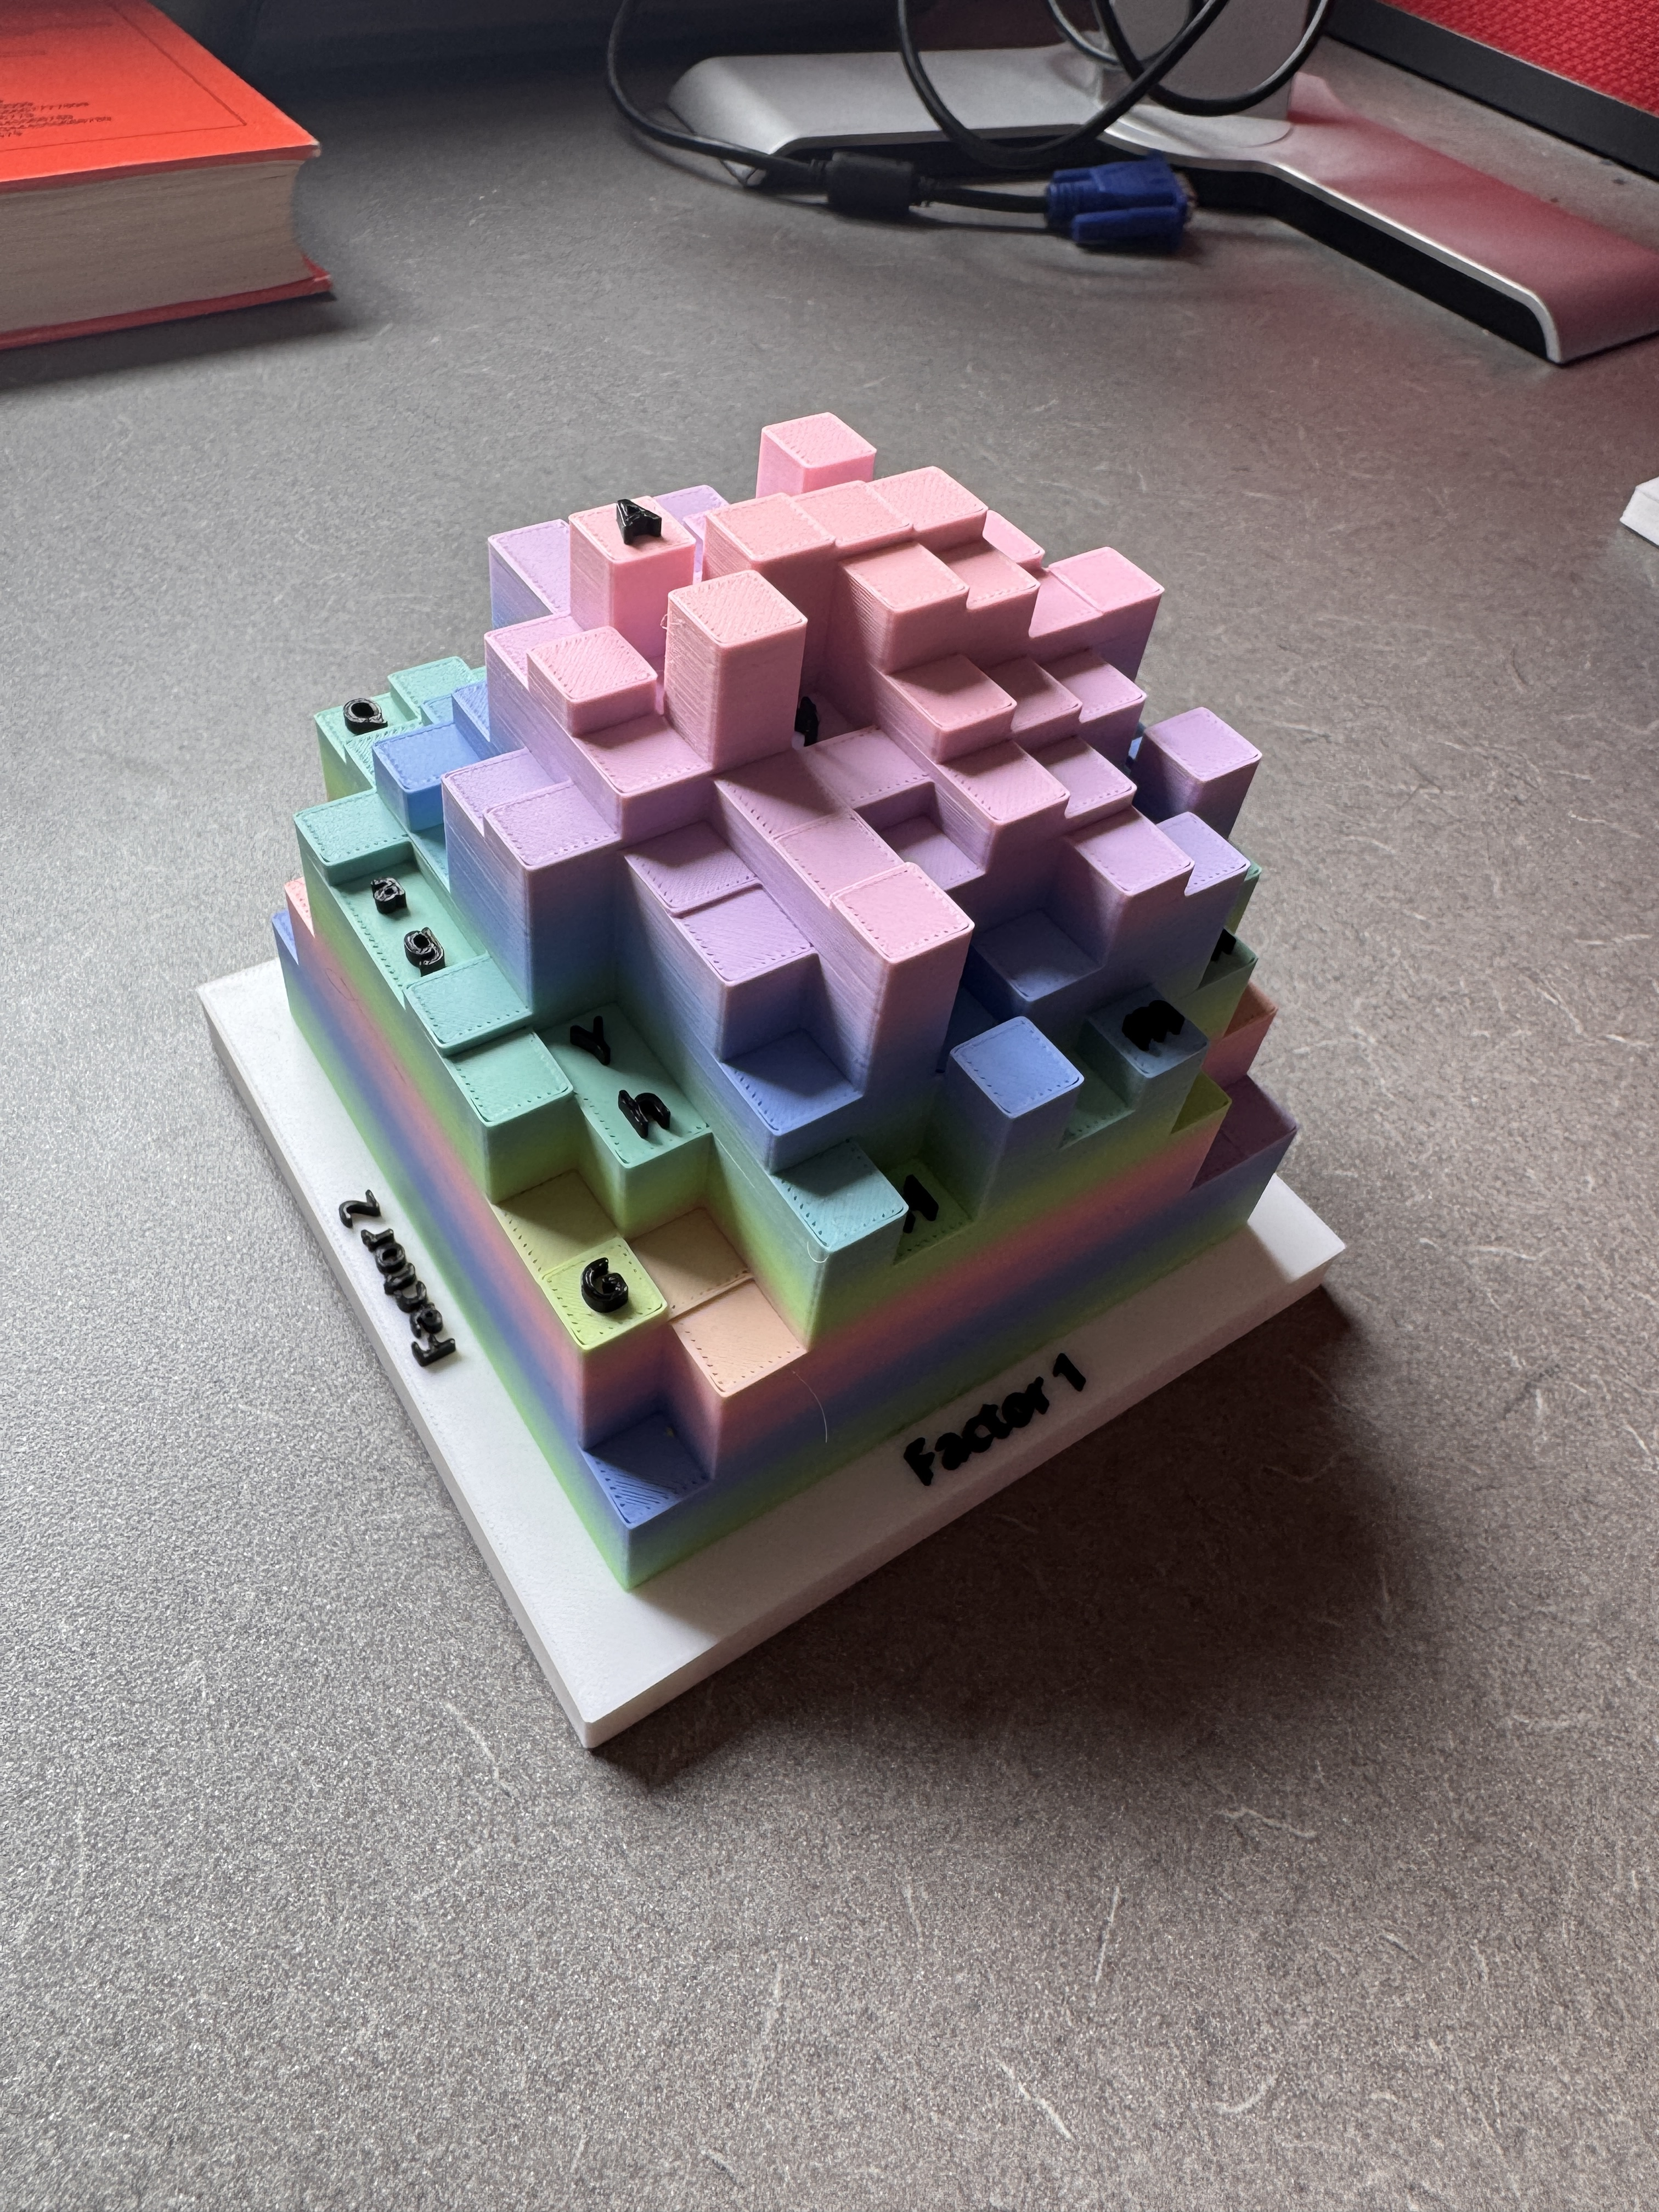
\includegraphics{images/3dp-gradient.JPG}

}

\subcaption{\label{fig-3dp-gradient}Solid filament of Data Set 1}

\end{minipage}%
%
\begin{minipage}{0.50\linewidth}

\centering{

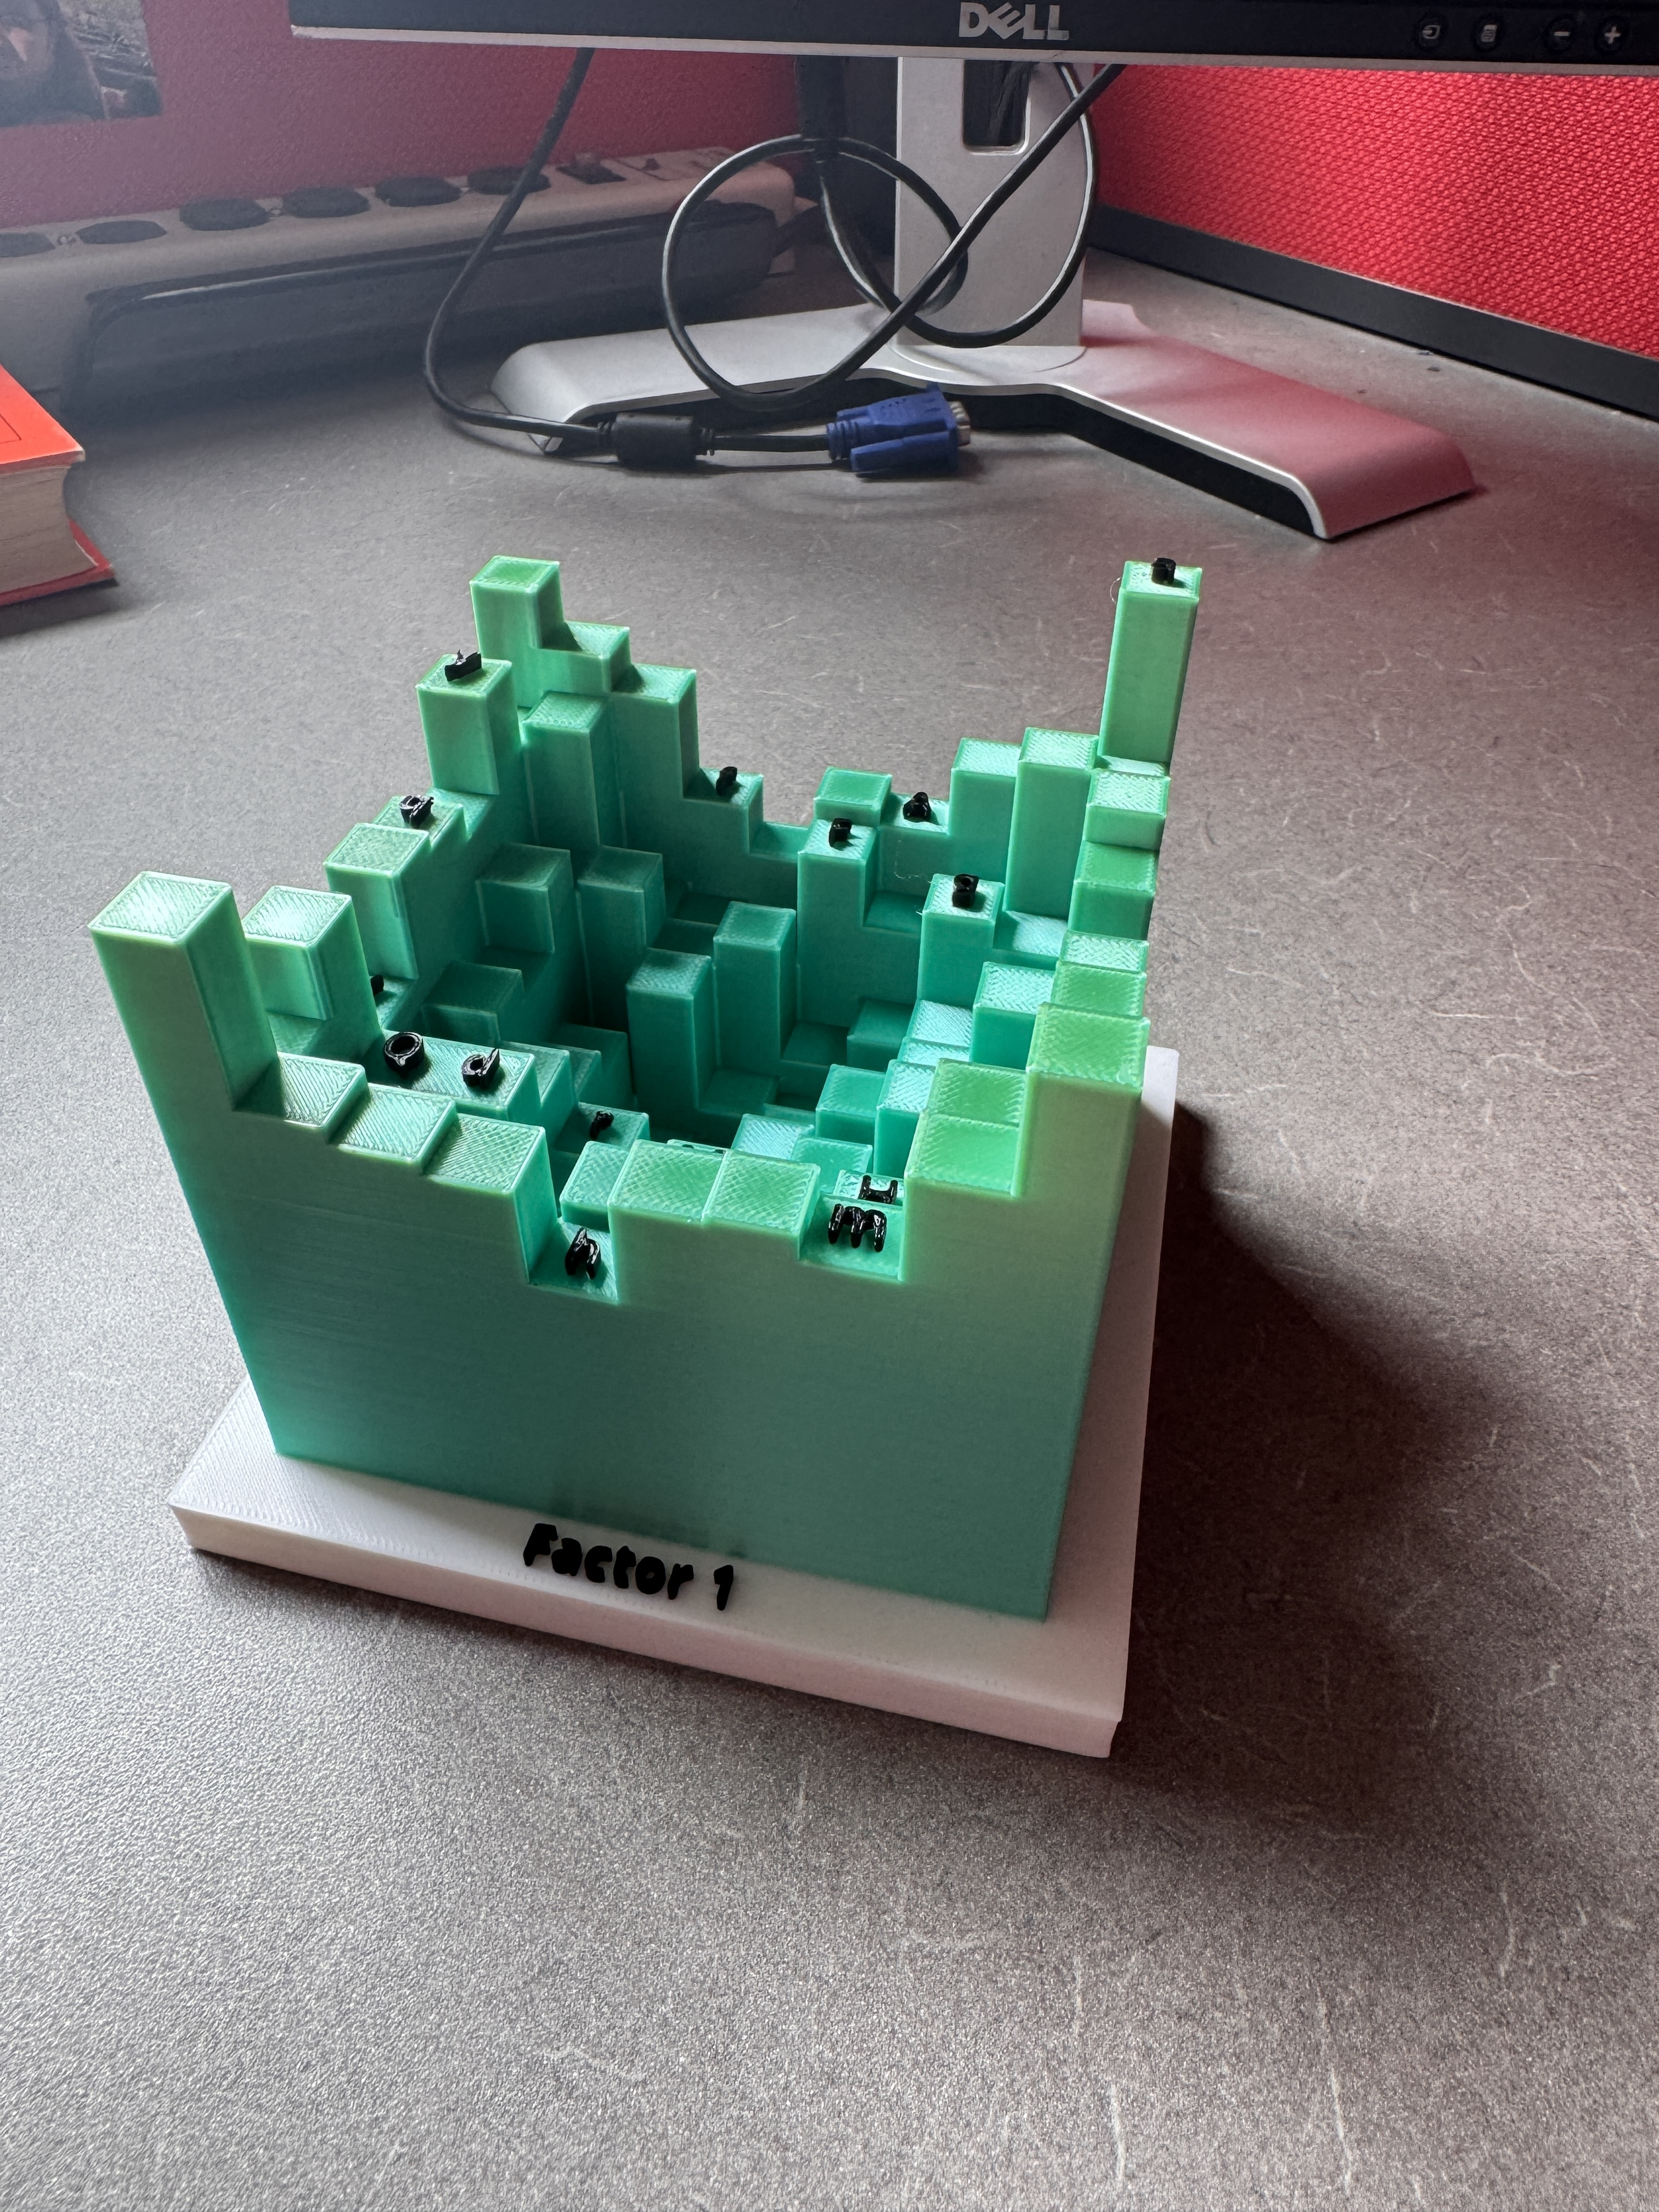
\includegraphics{images/3dp-solid.JPG}

}

\subcaption{\label{fig-3dp-solid}Solid filament of Data Set 2}

\end{minipage}%

\caption{\label{fig-3dp}3D printed heatmaps.}

\end{figure}%

To closely match the 3D-digital chart to the 3D-printed chart, multiple
stl files were created for each colored component and combined with the
RGL package (Murdoch and Adler 2023). The base was rendered with white
smoke (\#F5F5F5) to slightly contrast with the default white background
color (\#FFFFFF). Heatmap tiles were rendered with cyan (\#74CCFF) and
text labels were rendered with black (\#000000). Lighting was fixed at
45 degree angles at two opposite corners of the chart. The end result
was a near-perfect replica of the 3D-printed charts, with the exception
of different heatmap tile colors, where an example is given in
Figure~\ref{fig-3dd}.

\begin{figure}

\centering{

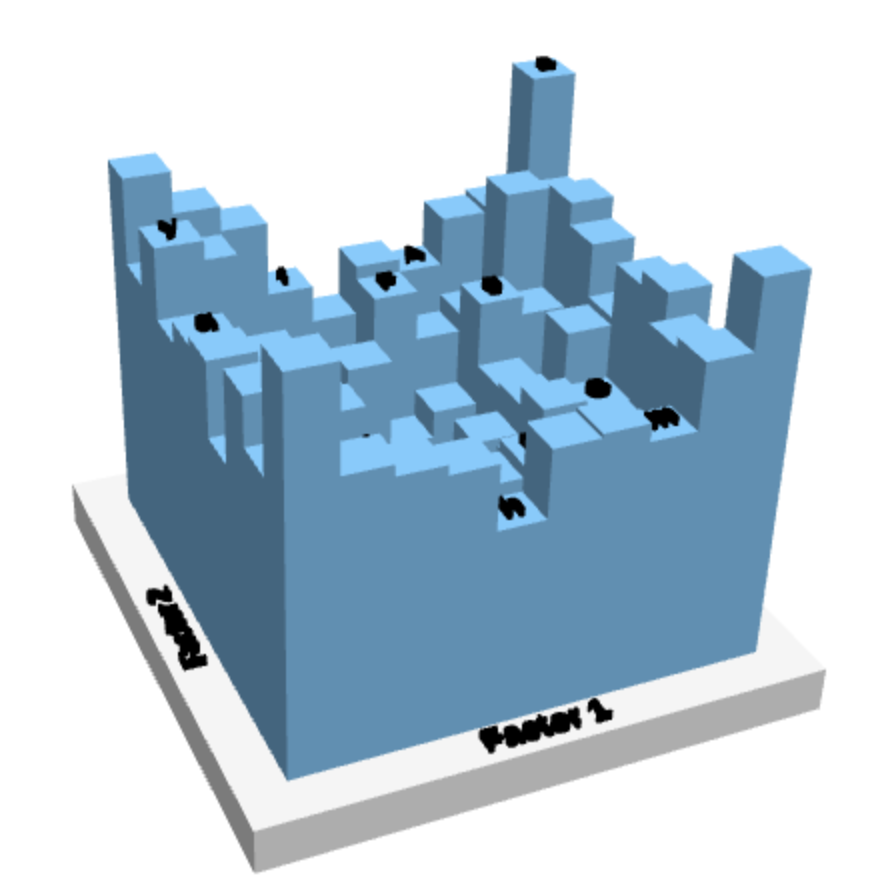
\includegraphics{images/chart-3dd.png}

}

\caption{\label{fig-3dd}RGL rendering of Data Set 2 for 3dd charts.}

\end{figure}%

Unlike the 3D charts, the 2D charts needed a different encoding to
convey heatmap values. The 2D heatmaps were created with
\texttt{ggplot2} (Wickham 2016) using \texttt{geom\_tile()}. Fill colors
for the cells use a color gradient ranging from Blue Zodiac (\#0C2841)
to Malibu (\#66D9FF), which were selected from a color picker using
shadows on our initial 3D-printed charts. The color interpolation was
performed with the \texttt{scale\_fill\_gradient()} function from the
\texttt{ggplot2} package.

\begin{figure}

\centering{


\includegraphics{index_files/figure-pdf/fig-color-pal-1.pdf}

}

\caption{\label{fig-color-pal}Color palette for 2D-digital charts. The
colors are interpolated from \#0C2841 to \#66D9FF, which are the colors
of the lighting conditions for a 3D-printed chart created with cyan
filament.}

\end{figure}%

\subsubsection{Subject Recruitment}\label{subject-recruitment}

Participants were recruited from all sections of STAT 218:
\emph{Introduction to Statistics} at the University of Nebraska-Lincoln
from June 2025 to December 2025. The experiment was incorporated into
the curriculum as a project that allowed students to get hands-on
experience with statistics. For data to be collected as part of our
study, students had to be at least 19 years of age and provide consent
to data collection.

STAT 218 is one of the possible courses under the general education
requirements for undergraduate degrees at the University of Nebraska. As
such, many students enrolled in the course are in the 18-25 age range
and are in the process of obtaining a Bachelor's degree. This allowed
for the unique opportunity for us to obtain a sample size that is
considerably larger than typical studies in graphical perception.

\subsubsection{Experimental Design}\label{experimental-design}

Our experiment was designed with a 3 x 2 x 9 treatment structure. Media
type is our main interest, with 2D-digital, 3D-digital, and 3D-printed
charts. To ensure that results are not confounded with datasets, we used
two datasets to create the heatmaps. A total of 9 stimuli pairs were
placed into each dataset. The order of treatments was given so that
media and dataset combinations were grouped together randomly in the
sequence and stimuli pairs were randomized within the groupings.

Due to practical constraints, stimuli pairs were incompletely blocked. A
full factorial design would result in 54 trials per participant, which
could lead to a decrease in quality responses (Herzog and Bachman 1981).
Therefore, we selected four out of the nine possible stimuli pairs to
create incomplete blocks. This resulted in 18 blocks for a balanced
incomplete block design. Within each block, media type is fully crossed
with dataset. Using the incomplete block structure, participants
completed a total of 24 trials, which is more practical than the full
factorial design. Blocks were chosen for each participant by using
probabilities that were proportional to the inverse counts of previously
chosen blocks. This ensured that blocks were approximately equally
distributed amongst the participants by increasing the probabilistic
weight of lesser chosen blocks.

Following the procedure of Cleveland and McGill (1984), we asked
participants two questions in each trial. The first question asked
participants which stimuli in a specified pair is larger or if the
stimuli are the same value. Next, participants were asked to estimate
the magnitude of the smaller stimuli if the larger stimuli represents
100 units, which is a subtractive process (Veit, n.d.). This question is
designed to estimate \(A/B\), where \(A\leq B\).

\paragraph{Shiny Application}\label{shiny-application}

A Shiny application (Chang et al. 2024) was developed to administer the
experiment. The application consisted of five sections: informed
consent, demographics, practice, experiment, and wrap-up. The entire
application was designed to be completed in approximately 30 minutes.

The Shiny application started with the informed consent screen, allowing
participants to select if they are a STAT 218 Student and if they agree
to the data collection. Participants had to select a data collection
option to continue. After submitting their data collection response, a
completion code was generated and saved on the last page of the
application. A copy of the informed consent is available in our GitHub
repository.

If participants agreed to have their data collected, they were presented
with the demographics section. This section asked participants to use
drop down menus to specify their age, gender identity, highest education
level, and a question about how their participation in the experiment is
graded. The last question was a text box and asked participants to
specify their favorite movie and/or actor. Demographic information was
combined with the application start time and completion code to create a
hash for an anonymized participant identifier using the \texttt{rlang}
package (Henry and Wickham 2025).

Once a participant completed the demographics page or selected ``No'' to
the data collection question, they were given a practice page. A modal
dialog window was initially shown with instructions, and users could
display this window again at any point during the practice trials. The
practice consisted of four questions: two trials from 2dd charts and two
trials from 3dd charts. Once participants provided a response to both
questions in a practice trial, they were able to display the correct
solution to check their answers.

The experiment page was presented to participants after completion of
the practice trials Figure~\ref{fig-exp-page}. Each page contained two
questions -- one question for identifying which stimuli is larger and
another question for estimating the value of the smaller stimuli if the
larger stimuli is 100 units. Each trial had the initial slider position
randomized in order to prevent starting position bias. For 3dd charts,
the number of interactive clicks was also recorded. A trial could only
be submitted if the first question is answered and if the slider was
moved at least once.

\begin{figure}

\centering{

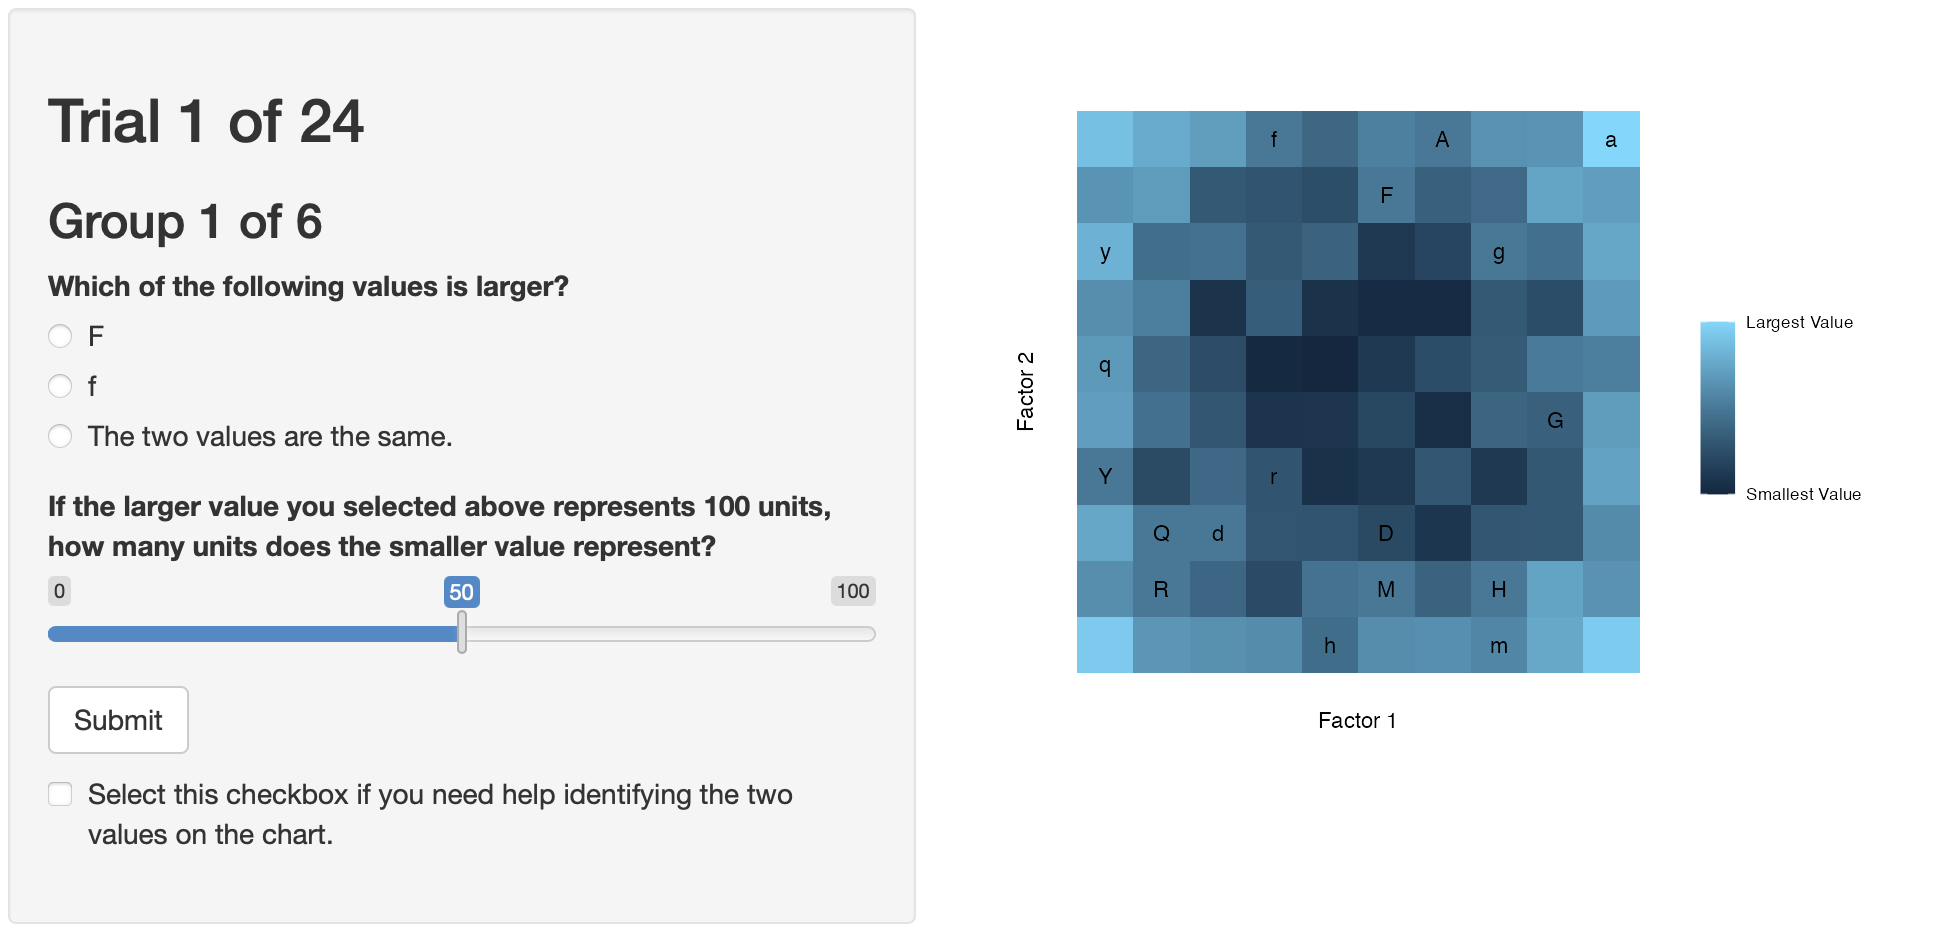
\includegraphics[width=1\textwidth,height=\textheight]{images/experiment-page.png}

}

\caption{\label{fig-exp-page}Graphics experiment page. Each trial
contained two questions about a pair of stimuli, and a check box that
displays the location of the stimuli if needed.}

\end{figure}%

After completing all trials, participants were given the completion code
and informed to provide the code to their instructor since they would
not have access to the code after closing out of the experiment.

\paragraph{Method of Analysis}\label{method-of-analysis}

The design of our experiment is a balanced incomplete split-plot with
replication, where media type and dataset are whole-plot factors for
each participant and stimuli pair is the split plot. A similar design
was presented by Mandal, Parsad, and Dash (2020) for a single replicate.
For our analysis, we used the following model as a baseline:

\[
Y_{ijklm}=\mu+S_i\times M_j\times P_k+\gamma_{lm}+\omega_{ijlm}+\epsilon_{ijklm}
\]

In our model, \(Y_ijklm\) is a metric of error for participant responses
to the ratio estimation question, \(S_i\) is the effect of dataset
\(i\), \(M_j\) is the effect of chart type \(j\), \(P_k\) is the effect
of stimuli pair \(k\), and \(S_i\times M_j\times P_k\) includes all
corresponding main effects and two-way and three-way interactions. Our
random effects include \(\gamma_{lm}\sim N(0,\sigma^2_A)\) for
participant \(m\) in block \(l\), \(\omega_{ijlm}\sim N(0,\sigma^2_B)\)
for the ordering of dataset \(i\) and chart type \(j\) for participant
\(m\) in block \(l\), and \(\epsilon_{ijklm}\sim N(0, \sigma^2_C)\) for
the residual error. We assume that \(\gamma_{lm}\), \(\omega_{ijlm}\),
and \(\epsilon_{ijklm}\) are independently and identically distributed.

The first question in each trial was to indicate which value within a
stimulus pair was larger, or if they were the same value. Following
Cleveland and McGill (1984), we use this question as an attention check
to verify that participants are following the procedure and that the
correct comparison is being made.

\subsection{Results}\label{results}

In this section, we describe the demographic information of our sample,
cleaning of participant responses, analysis of responses, and
interactions participants had with the Shiny application.

\subsubsection{Demographics}\label{demographics}

Our experiment was conducted with eight sections of Stat 218 between
August 25th and December 19th in 2025 at the University of Nebraska. To
participate in the experiment, students were instructed to visit
communal office hour locations to access the 3D printed charts. We
recorded 482 interactions with the shiny application, of which 259
students completed the entirety of the experiment. Of these students, 92
were enrolled in online sections of the course and did not have access
to the 3D printed charts. The vast majority of participants were
actively completing their undergraduate degree and between the ages of
19 and 25. Full demographic information can be found in
Table~\ref{tbl-demographics}.

\begin{table}

\caption{\label{tbl-demographics}}

\centering{

\centering
\caption{Demographic Information}
\centering
\begin{tabular}[t]{lrr}
\toprule
 & Count & Proportion\\
\midrule
\addlinespace[0.3em]
\multicolumn{3}{l}{\textbf{Gender}}\\
\hspace{1em}Female & 166 & 0.64\\
\hspace{1em}Male & 90 & 0.35\\
\hspace{1em}Variant/Nonconforming & 1 & 0.00\\
\hspace{1em}Prefer not to answer & 2 & 0.01\\
\addlinespace[0.3em]
\multicolumn{3}{l}{\textbf{Age}}\\
\hspace{1em}19-25 & 252 & 0.97\\
\hspace{1em}26-30 & 2 & 0.01\\
\hspace{1em}31-35 & 0 & 0.00\\
\hspace{1em}36-40 & 1 & 0.00\\
\hspace{1em}41-45 & 3 & 0.01\\
\hspace{1em}Prefer not to answer & 1 & 0.00\\
\addlinespace[0.3em]
\multicolumn{3}{l}{\textbf{Education}}\\
\hspace{1em}High School or Less & 23 & 0.09\\
\hspace{1em}Some Undergraduate Courses & 214 & 0.83\\
\hspace{1em}Undergraduate Degree & 12 & 0.05\\
\hspace{1em}Some Graduate Courses & 4 & 0.02\\
\hspace{1em}Graduate Degree & 2 & 0.01\\
\hspace{1em}Prefer not to answer & 4 & 0.02\\
\bottomrule
\end{tabular}

}

\end{table}%

Almost all participants completed the experiment in under 20 minutes.
Summary statistics can be found in Table~\ref{tbl-exp-times}, with the
overall distribution of times shown in Figure~\ref{fig-total-time}.
Individual trials had a median completion time of 0.23 minutes.

\begin{longtable}[]{@{}lrrr@{}}

\caption{\label{tbl-exp-times}Summary of experiment completion times in
minutes.}

\tabularnewline

\toprule\noalign{}
Section & Mean & SD & Median \\
\midrule\noalign{}
\endhead
\bottomrule\noalign{}
\endlastfoot
In-person & 8.08 & 3.39 & 7.45 \\
Online & 5.70 & 3.42 & 5.09 \\
All Participants & 7.23 & 3.58 & 6.86 \\

\end{longtable}

\begin{figure}

\centering{

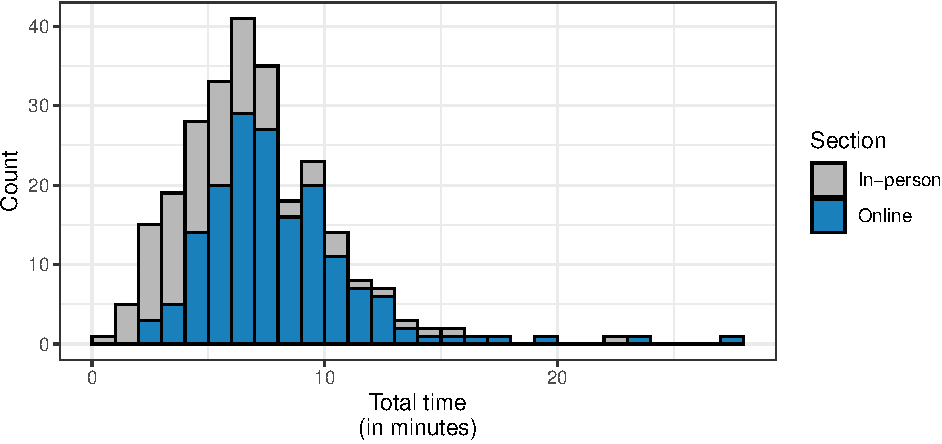
\includegraphics{index_files/figure-pdf/fig-total-time-1.pdf}

}

\caption{\label{fig-total-time}Histogram of experiment completion times.
Online participants had generally shorter completion times due to a
decreased number of trials.}

\end{figure}%

During our initial exploration of the results, we discovered a
non-negligible number of students who did not follow the instructions.
In some cases, participants appeared to be using alternative estimation
strategies, such as estimating the difference between the two values in
a stimulus pair. Additionally, we noticed that several students were
randomly entering values in order to obtain the completion code at the
end of the experiment. We provide some examples of individual
participant responses in Figure~\ref{fig-user-strategies} to illustrate
this issue.

\begin{figure}

\centering{

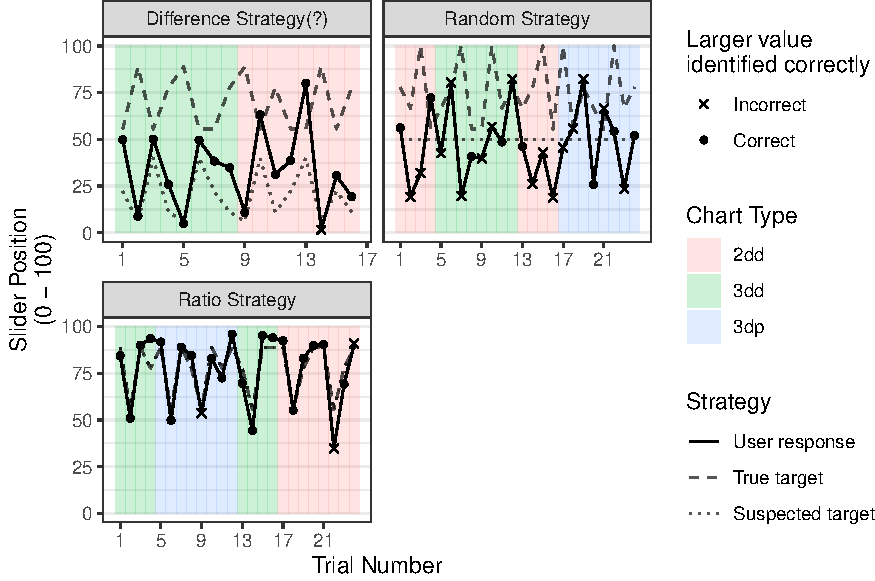
\includegraphics{index_files/figure-pdf/fig-user-strategies-1.pdf}

}

\caption{\label{fig-user-strategies}Three potential estimation
strategies from participants. Many participants followed instructions to
estimate ratios. However, some participants appeared to estimate the
difference between stimuli pairs or submitted random values.}

\end{figure}%

It is commonly acknowledged in psychology that careless respondents
should be addressed to some degree, although there is no general
consensus on how to handle this in recent years (Jaso, Kraus, and Heller
2021; Ward and Meade 2023). Some proposed solutions include removing
participants based on observed patterns or fitting mixture models to
address latent class variables. In this section, we discuss one possible
subset of participant responses to address careless respondents. We also
include the models of several other subsets in the appendix.

\subsubsection{Addressing Random Categorical
Responses}\label{sec-remove-random-categories}

To improve the quality of our data, we started by assessing random
guesses in identifying the larger value of a stimulus pair. In each
trial, participants have a 1/3 probability of correctly identifying the
larger value if they are randomly guessing. Since stimuli pair 5
contains identical values, we temporarily exclude those trials to focus
on stimuli pairs where there was a difference between the values. For
each participant, we test \(H_0: \pi\leq2/3\text{ vs. }H_1:\pi>2/3\)
with \(\alpha=0.05\), where \(\pi\) is the probability of a participant
correctly answering the initial question and \(\alpha\) is the level of
the test. Using the first question for participant screening, 5311
participants are excluded for suspected random selecting, leaving 161
participants. The effect of this exclusion can be seen in
Figure~\ref{fig-q1-eda}.

\begin{figure}

\begin{minipage}{0.50\linewidth}

\centering{

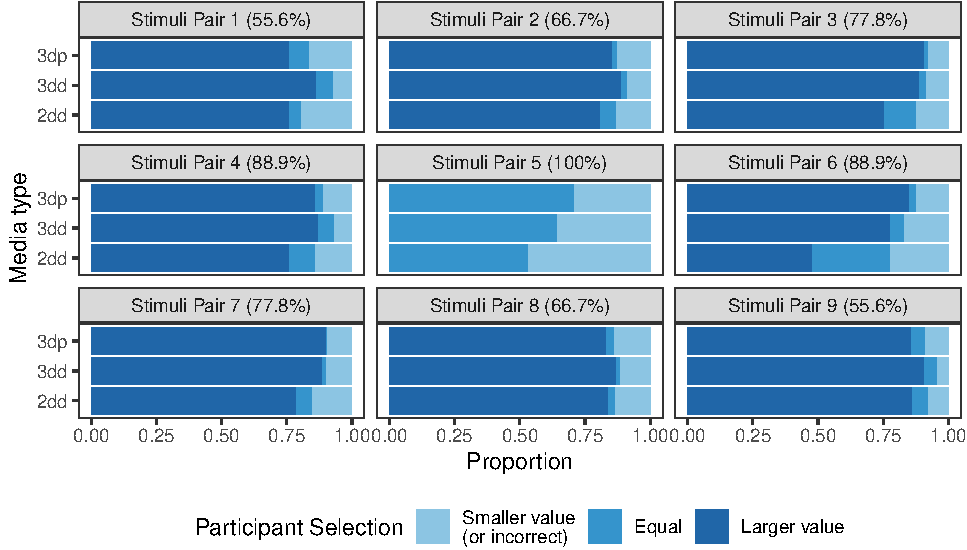
\includegraphics[width=0.9\textwidth,height=\textheight]{index_files/figure-pdf/fig-q1-eda-1.pdf}

}

\subcaption{\label{fig-q1-eda-1}No participant filtering}

\end{minipage}%
%
\begin{minipage}{0.50\linewidth}

\centering{

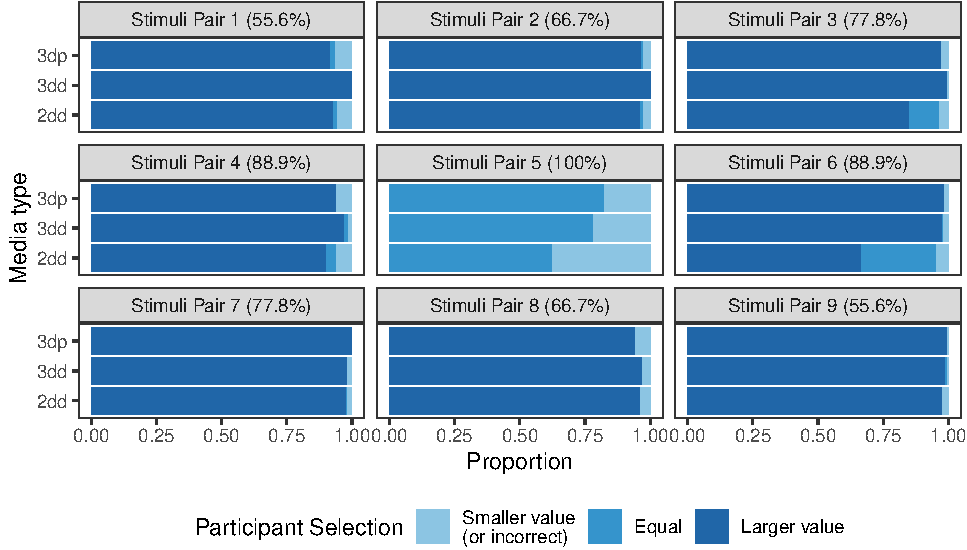
\includegraphics[width=0.9\textwidth,height=\textheight]{index_files/figure-pdf/fig-q1-eda-2.pdf}

}

\subcaption{\label{fig-q1-eda-2}Exclude random guessers}

\end{minipage}%

\caption{\label{fig-q1-eda}Proportion of correct responses to Question 1
across stimuli pairs and media types. For all pairs, with the exception
of Pair 5, a correct answer was `Larger value'. Stimuli Pair 5 had two
identical values, meaning that options other than `Both values are the
same' were incorrect.}

\end{figure}%

\subsubsection{Analysis of Error}\label{analysis-of-error}

We follow the same calculation of error as Cleveland and McGill (1984),
which is shown in Equation~\ref{eq-error_cm}. Error is defined as the
base-2 logarithm of the absolute estimation error meaning that
differences of one unit on this scale correspond to approximately
doubling the size of the error. The addition of 1/8 prevents distortion
for responses with near-zero error.

\begin{equation}\phantomsection\label{eq-error_cm}{
y=\log_2(|\text{User Response}-100\times(\text{True ratio})|+1/8)
}\end{equation}

In our analysis, we excluded individual responses where participants
were incorrect in their response to the initial question and all
responses for stimuli pair 5. The initial question served as an
attention check to verify that the participants were making the correct
comparison between stimuli values. For stimuli pair 5, we removed these
trials since correct solutions should be a binary response. However, we
discovered a discrepancy in how participants were responding to both
questions for these trials, which we discuss in the appendix.

With our specified exclusion criteria, we find that there was marginal
evidence for the effects of chart type (p-value = 0.041) and the data
set and stimuli pair interaction (p-value = 0.073). This finding is
consistent with models fitted with various participant and response
filters.

Our findings showed that the 2D heatmaps had evidence of higher log
absolute error than both types of the 3D heatmaps. On the base-2 log
scale, the error for 2D heatmaps was larger than the error for digital
3D heatmap by 0.414 (95\% CI: 0.253, 0.574). This finding is similar for
the 3D printed heatmaps, where the log absolute error for 2D heatmaps
was larger by 0.413 (95\% CI: 0.234, 0.591). There were no detectable
differences in error between the digital and physical 3D heatmaps
(p-value = 1).

\begin{figure}

\centering{

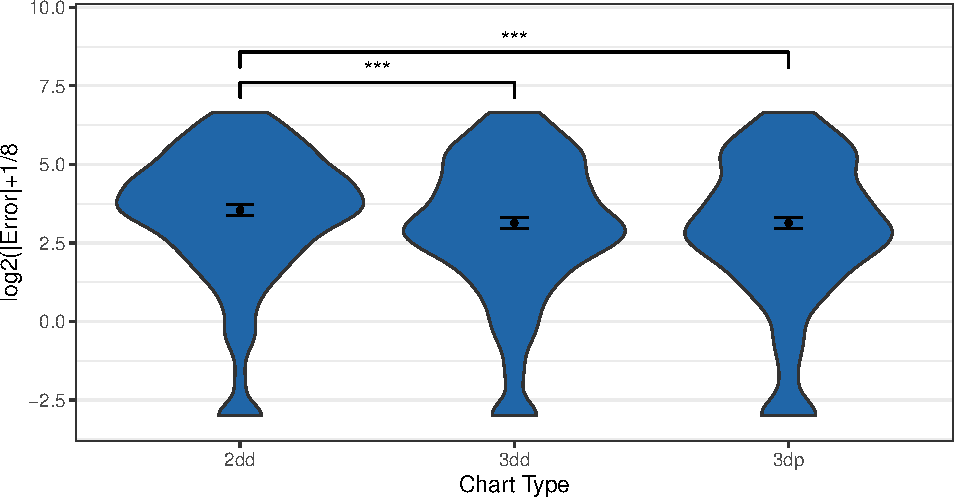
\includegraphics{index_files/figure-pdf/fig-em-media-1.pdf}

}

\caption{\label{fig-em-media}Estimated marginal means of chart type.
Differences were only detected between 2D heatmap and both types of 3D
heatmaps, where the 2D heatmap had evidence of larger errors.}

\end{figure}%

When examining the interaction between stimuli pairs and underlying
datasets, 11 differences in log absolute error were detected at the
\(\alpha=0.05\) level. Seven of these differences occurred with stimuli
pair 6 (ratio = 0.889) and dataset 1, which had the smallest estimated
marginal mean of log absolute error. All differences can be found in
Figure~\ref{fig-em-set-pair}, where significant differences are assessed
via a compact letter display from the \texttt{multcomp} package
(\textbf{multcomp?}).

\begin{figure}

\centering{

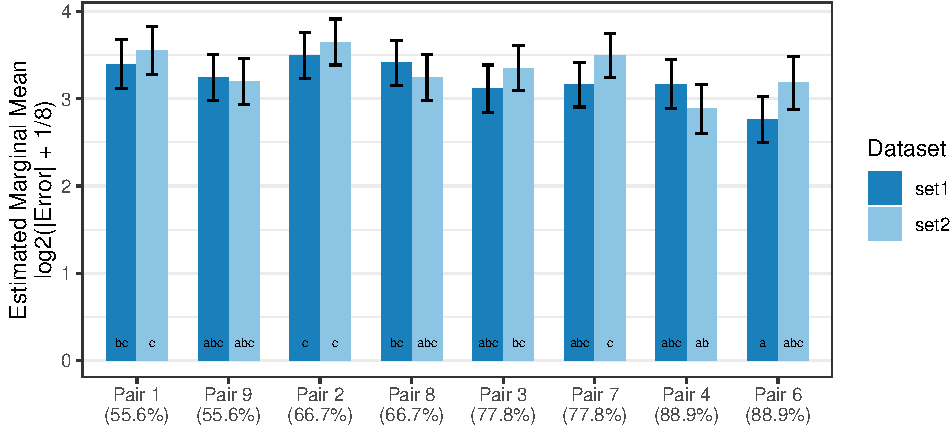
\includegraphics{index_files/figure-pdf/fig-em-set-pair-1.pdf}

}

\caption{\label{fig-em-set-pair}Estimated marginal means of stimuli pair
and dataset. Bars sharing the same letter are not significantly
different from one another.}

\end{figure}%

\subsubsection{Participant Interactions with Shiny
Application}\label{participant-interactions-with-shiny-application}

In this section, we describe participant interactions with the Shiny
application using the same participant exclusion criteria as our model.
As participants completed the experiment, we recorded the amount of time
to complete each trial, the number of cursor clicks on the digital 3D
heatmaps, and the number of times that the slider was moved. We also
recorded the initial starting position of the slider, which was randomly
placed for each trial.

Many participants completed each trial in under 20 seconds. The median
completion time was 14.8372396 seconds, with a standard deviation of
22.9971286 seconds. There were 91 participants who had at least one
trial exceed 60 seconds. Due to the design of the administration of the
experiment, we are unable to account for the cause of longer trial
completion times.

\begin{figure}

\begin{minipage}{0.50\linewidth}

\centering{

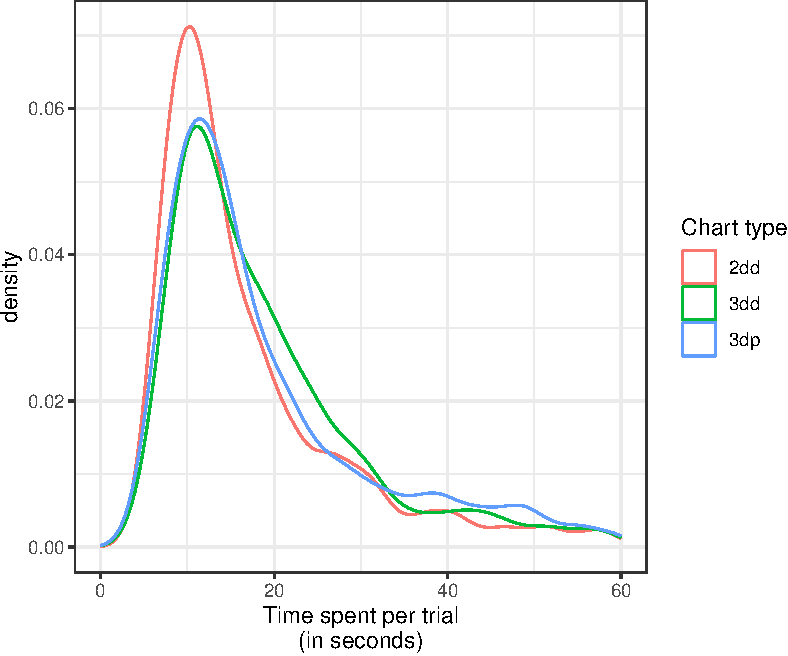
\includegraphics[width=0.9\textwidth,height=\textheight]{index_files/figure-pdf/fig-time-summary-1.pdf}

}

\subcaption{\label{fig-time-summary-1}Frequency plot}

\end{minipage}%
%
\begin{minipage}{0.50\linewidth}

\centering{

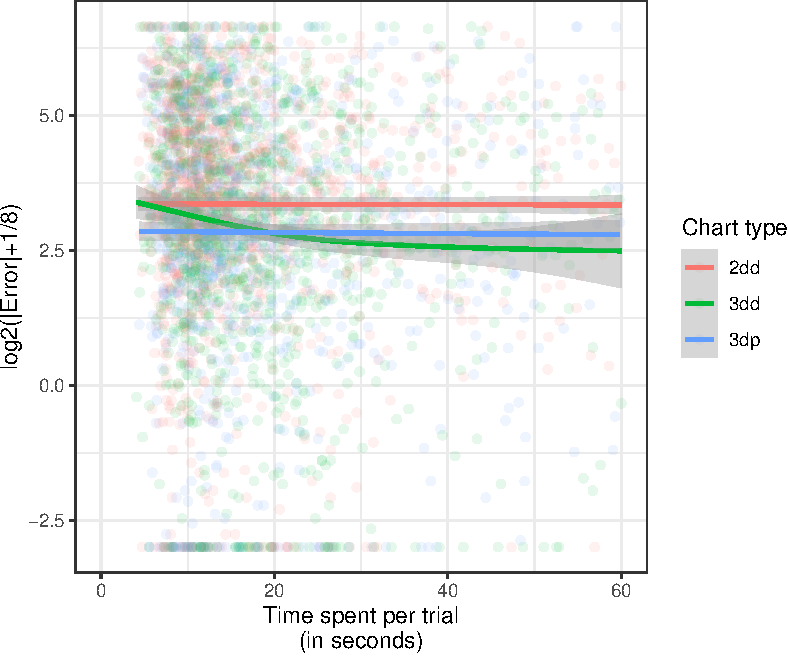
\includegraphics[width=0.9\textwidth,height=\textheight]{index_files/figure-pdf/fig-time-summary-2.pdf}

}

\subcaption{\label{fig-time-summary-2}Time vs.~Error}

\end{minipage}%

\caption{\label{fig-time-summary}Visual summary of time spent on each
trial. 137 trials are omitted due to lasting longer than 60 seconds.}

\end{figure}%

\begin{figure}

\begin{minipage}{0.50\linewidth}

\centering{

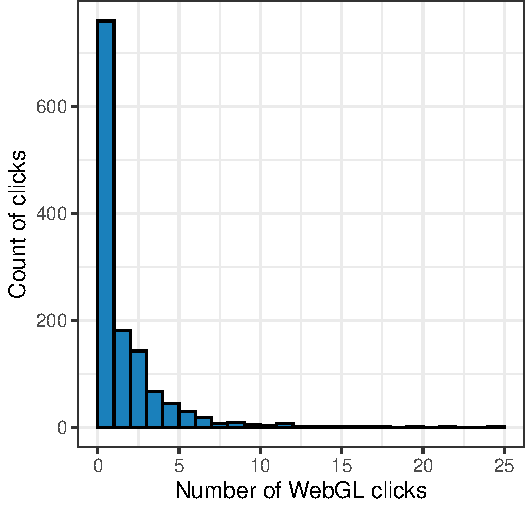
\includegraphics[width=0.9\textwidth,height=\textheight]{index_files/figure-pdf/fig-clicks3dd-1.pdf}

}

\subcaption{\label{fig-clicks3dd-1}Histogram}

\end{minipage}%
%
\begin{minipage}{0.50\linewidth}

\centering{

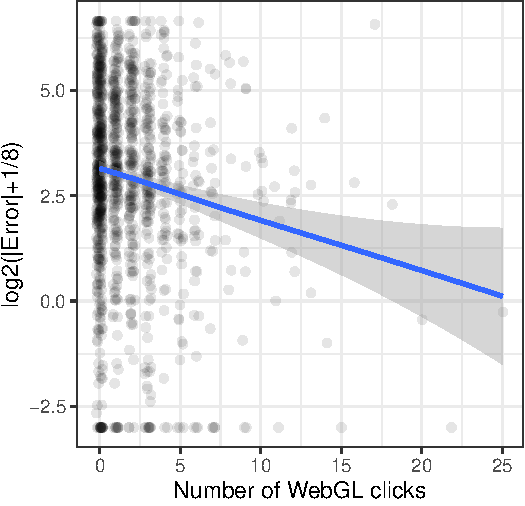
\includegraphics[width=0.9\textwidth,height=\textheight]{index_files/figure-pdf/fig-clicks3dd-2.pdf}

}

\subcaption{\label{fig-clicks3dd-2}WebGL clicks vs.~Error}

\end{minipage}%

\caption{\label{fig-clicks3dd}Participant interactions with the digital
3D heatmaps.}

\end{figure}%

\begin{figure}

\begin{minipage}{0.50\linewidth}

\centering{

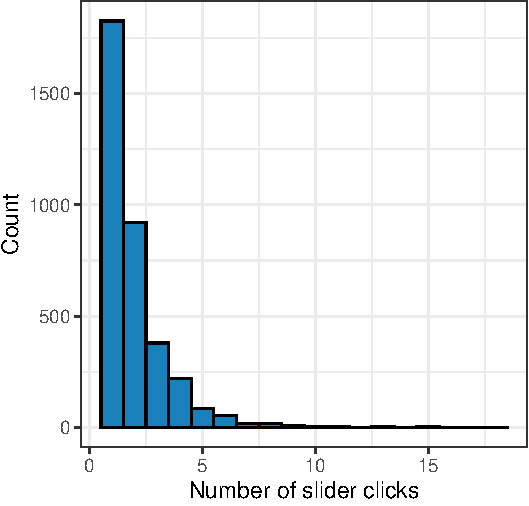
\includegraphics[width=0.9\textwidth,height=\textheight]{index_files/figure-pdf/fig-slider-clicks-1.pdf}

}

\subcaption{\label{fig-slider-clicks-1}Histogram}

\end{minipage}%
%
\begin{minipage}{0.50\linewidth}

\centering{

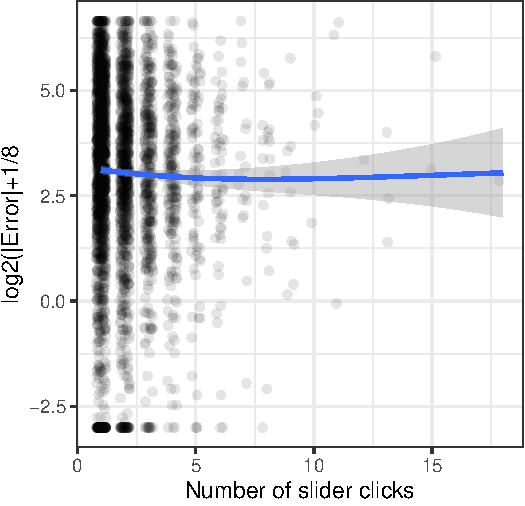
\includegraphics[width=0.9\textwidth,height=\textheight]{index_files/figure-pdf/fig-slider-clicks-2.pdf}

}

\subcaption{\label{fig-slider-clicks-2}Slider clicks vs.~Error}

\end{minipage}%

\caption{\label{fig-slider-clicks}Participant interactions with the
slider.}

\end{figure}%

\begin{figure}

\centering{

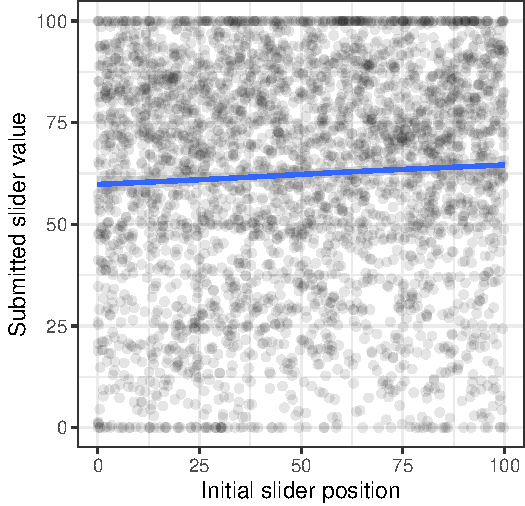
\includegraphics{index_files/figure-pdf/fig-slider-start-1.pdf}

}

\caption{\label{fig-slider-start}Effect of initial slider position on
the submitted slider value.}

\end{figure}%

\subsection{Discussion and Conclusion}\label{discussion-and-conclusion}

Our study was designed to test the numerical estimation of ratios in 2D
and 3D heatmaps rendered in digital and physical environments. The
current state of tangible statistical graphics is limited mainly to
tactile displays, whereas 3D printed statistical graphics are largely
unexplored. We found that when the third dimension is conveying
meaningful information, the heights of 3D heatmaps had smaller errors
than the color gradient of 2D heatmaps. No differences were detected
between the digital and physical 3D heatmaps, which is perhaps
attributed to the exact one-to-one design relationship between the
digital display and the 3D printed chart.

An interesting observation from the stimuli pairs and dataset
interaction was from the non-detectable differences. We note that no
differences were detected across datasets for a given stimuli pair.
While not explicitly tested in our experiment, there have been previous
studies that have investigated and found the behavior of neighboring
values to have an effect (Zacks et al. 1998;
\textbf{vanderplasSignsSineIllusion2015?}). This effect would be worth
exploring in future studies with 3D heatmaps. Another concern we had
when designing our experiment was the lack of direct translation from
color scales to heights. The differences between stimuli pairs of
identical ratios were non-detectable, which alleviates this concern for
future studies. However, this effect would likely important to consider
if assessing just noticeable differences
(\textbf{luModelingJustNoticeable2022?};
\textbf{zhangJustNoticeableDifference2023?}).

While our hypothesis that 3D-printed heatmaps would outperform digital
2D and 3D heat maps in numerical estimations of ratios was not
supported, we were able to show that 3D charts have a place in the
analysis of data. When the third dimension is used to display
information, the mapping of that dimension to height provides better
ratio estimations than a color gradient scale. This result has been
observed previously in digital 3D heatmaps (Barfield and Robless 1989;
Kraus et al. 2020), and our findings suggests that this holds for
physical 3D heatmaps.

\subsection{Appendix}\label{appendix}

In this section, we include multiple models for the transparency of
model selection. Visual inspections of participant responses indicate
that several participants clearly did not follow instructions by either
using alternate estimation strategies or by carelessly responding
Figure~\ref{fig-q1-eda}. While we should take these cases into
consideration, there is no singular solution to suggest a ``best'' model
(Jaso, Kraus, and Heller 2021; Ward and Meade 2023). Our purpose for
including these alternate models is to examine model sensitivity to
results through various levels of participant and response filtering.

For each model, we exclude stimuli pair 5. In theory, participants who
answer this question correctly will select that both values are the same
and move the slider to 100. From the included participants, as described
in Section~\ref{sec-remove-random-categories}, virtually all
participants who put the slider at 100 answered the first question
correctly. However, nearly 60 percent of responses indicated that the
values were the same in the first question but did not move the slider
to 100. Several factors could have attributed to this, such as slider
sensitivity or participants using alternate estimation strategies.
Rather than correcting what we think participants should have answered,
we removed this stimuli pair and motivate future research into ``just
noticeable differences'' for 3D heatmaps.

\begin{figure}

\centering{


\includegraphics{index_files/figure-pdf/fig-pair5-issues-1.pdf}

}

\caption{\label{fig-pair5-issues}Counts of response behavior for when
values in the stimuli pair were the same.}

\end{figure}%

There are multiple levels of participant and response filtering that we
considered. For participant filtering, we consider the following levels:
(1) no participant filtering and (2) remove suspected random guessers.
The process of (2) was described in
Section~\ref{sec-remove-random-categories}. Filtering individual
responses is a straightforward process, where we considered (i) include
all responses, and (ii) remove responses with incorrect Q1 solutions.

\begin{longtable}[]{@{}
  >{\raggedright\arraybackslash}p{(\columnwidth - 14\tabcolsep) * \real{0.3333}}
  >{\raggedleft\arraybackslash}p{(\columnwidth - 14\tabcolsep) * \real{0.0541}}
  >{\raggedleft\arraybackslash}p{(\columnwidth - 14\tabcolsep) * \real{0.0541}}
  >{\raggedleft\arraybackslash}p{(\columnwidth - 14\tabcolsep) * \real{0.0721}}
  >{\raggedleft\arraybackslash}p{(\columnwidth - 14\tabcolsep) * \real{0.0901}}
  >{\raggedleft\arraybackslash}p{(\columnwidth - 14\tabcolsep) * \real{0.1081}}
  >{\raggedleft\arraybackslash}p{(\columnwidth - 14\tabcolsep) * \real{0.1261}}
  >{\raggedleft\arraybackslash}p{(\columnwidth - 14\tabcolsep) * \real{0.1622}}@{}}
\caption{ANOVA p-values for different effects}\tabularnewline
\toprule\noalign{}
\begin{minipage}[b]{\linewidth}\raggedright
model
\end{minipage} & \begin{minipage}[b]{\linewidth}\raggedleft
set
\end{minipage} & \begin{minipage}[b]{\linewidth}\raggedleft
media
\end{minipage} & \begin{minipage}[b]{\linewidth}\raggedleft
pair\_id
\end{minipage} & \begin{minipage}[b]{\linewidth}\raggedleft
set:media
\end{minipage} & \begin{minipage}[b]{\linewidth}\raggedleft
set:pair\_id
\end{minipage} & \begin{minipage}[b]{\linewidth}\raggedleft
media:pair\_id
\end{minipage} & \begin{minipage}[b]{\linewidth}\raggedleft
set:media:pair\_id
\end{minipage} \\
\midrule\noalign{}
\endfirsthead
\toprule\noalign{}
\begin{minipage}[b]{\linewidth}\raggedright
model
\end{minipage} & \begin{minipage}[b]{\linewidth}\raggedleft
set
\end{minipage} & \begin{minipage}[b]{\linewidth}\raggedleft
media
\end{minipage} & \begin{minipage}[b]{\linewidth}\raggedleft
pair\_id
\end{minipage} & \begin{minipage}[b]{\linewidth}\raggedleft
set:media
\end{minipage} & \begin{minipage}[b]{\linewidth}\raggedleft
set:pair\_id
\end{minipage} & \begin{minipage}[b]{\linewidth}\raggedleft
media:pair\_id
\end{minipage} & \begin{minipage}[b]{\linewidth}\raggedleft
set:media:pair\_id
\end{minipage} \\
\midrule\noalign{}
\endhead
\bottomrule\noalign{}
\endlastfoot
All participants, all responses & 0.340 & 0.010 & 0.244 & 0.297 & 0.003
& 0.815 & 0.489 \\
All participants, Q1 correct & 0.705 & 0.018 & 0.333 & 0.711 & 0.145 &
0.740 & 0.764 \\
Filtered participants, all responses & 0.939 & 0.035 & 0.089 & 0.543 &
0.001 & 0.982 & 0.255 \\
Filtered participants, Q1 correct & 0.735 & 0.041 & 0.063 & 0.669 &
0.073 & 0.968 & 0.833 \\
\end{longtable}

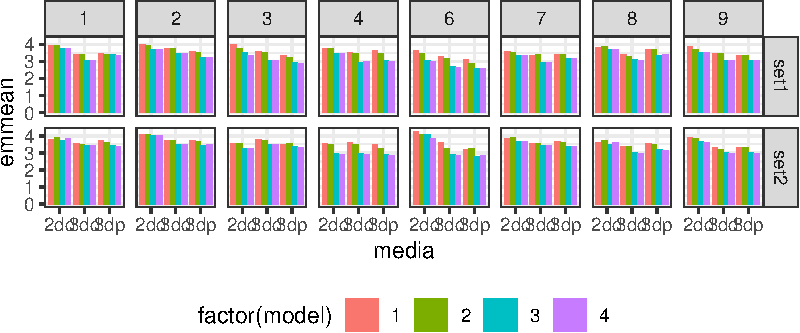
\includegraphics{index_files/figure-pdf/unnamed-chunk-18-1.pdf}

In addition to our parametric methods, we also present the results of a
generalized additive model in Equation~\ref{eq-gam}

\begin{tcolorbox}[enhanced jigsaw, leftrule=.75mm, colframe=quarto-callout-note-color-frame, toptitle=1mm, bottomtitle=1mm, colbacktitle=quarto-callout-note-color!10!white, left=2mm, bottomrule=.15mm, opacitybacktitle=0.6, arc=.35mm, breakable, title=\textcolor{quarto-callout-note-color}{\faInfo}\hspace{0.5em}{Note}, opacityback=0, coltitle=black, rightrule=.15mm, toprule=.15mm, colback=white, titlerule=0mm]

I adapted code from our first paper, but I would like a second look over
this model before writing it up. The good news is that the results seem
to be similar :)

\end{tcolorbox}

\begin{equation}\phantomsection\label{eq-gam}{
\text{MODEL GOES HERE}
}\end{equation}

\begin{verbatim}

Family: gaussian 
Link function: identity 

Formula:
q2_error_cm ~ set * media + s(target_ratio, k = 4, by = media) + 
    s(target_ratio, k = 4, by = set) + s(user_id, bs = "re")

Parametric Terms:
          df      F  p-value
set        1  0.281    0.596
media      2 13.631 1.28e-06
set:media  2  0.448    0.639

Approximate significance of smooth terms:
                              edf   Ref.df     F p-value
s(target_ratio):media2dd   0.8001   0.8001 5.918  0.0296
s(target_ratio):media3dd   0.8000   0.8000 0.005  0.9481
s(target_ratio):media3dp   0.8000   0.8000 0.835  0.4138
s(target_ratio):setset1    2.0434   2.4098 4.168  0.0155
s(target_ratio):setset2    2.1097   2.4698 6.755  0.0137
s(user_id)               139.2678 160.0000 7.088  <2e-16
\end{verbatim}

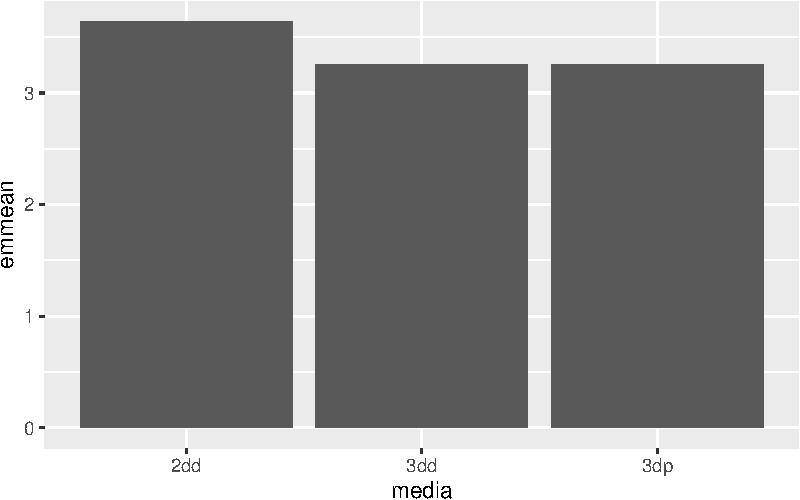
\includegraphics{index_files/figure-pdf/unnamed-chunk-19-1.pdf}

\newpage

\subsection{References}\label{references}

\phantomsection\label{refs}
\begin{CSLReferences}{1}{0}
\bibitem[\citeproctext]{ref-barfield1989}
Barfield, Woodrow, and Robert Robless. 1989. {``The Effects of Two- or
Three-Dimensional Graphics on the Problem-Solving Performance of
Experienced and Novice Decision Makers.''} \emph{Behaviour \&
Information Technology} 8 (5): 369--85.
\url{https://doi.org/10.1080/01449298908914567}.

\bibitem[\citeproctext]{ref-shiny}
Chang, Winston, Joe Cheng, JJ Allaire, Carson Sievert, Barret Schloerke,
Yihui Xie, Jeff Allen, Jonathan McPherson, Alan Dipert, and Barbara
Borges. 2024. {``Shiny: Web Application Framework for r.''}
\url{https://shiny.posit.co/}.

\bibitem[\citeproctext]{ref-cleveland1984}
Cleveland, William S., and Robert McGill. 1984. {``Graphical Perception:
Theory, Experimentation, and Application to the Development of Graphical
Methods.''} \emph{Journal of the American Statistical Association} 79
(387): 531--54. \url{https://doi.org/10.1080/01621459.1984.10478080}.

\bibitem[\citeproctext]{ref-croxton1927}
Croxton, Frederick E., and Roy E. Stryker. 1927. {``Bar Charts Versus
Circle Diagrams.''} \emph{Journal of the American Statistical
Association} 22 (160): 473--82. \url{https://doi.org/10.2307/2276829}.

\bibitem[\citeproctext]{ref-eells1926}
Eells, Walter Crosby. 1926. {``The Relative Merits of Circles and Bars
for Representing Component Parts.''} \emph{Journal of the American
Statistical Association} 21 (154): 119--32.
\url{https://doi.org/10.1080/01621459.1926.10502165}.

\bibitem[\citeproctext]{ref-fischer2000}
Fischer, Martin H. 2000. {``Do Irrelevant Depth Cues Affect the
Comprehension of Bar Graphs?''} \emph{Applied Cognitive Psychology} 14
(2): 151--62.
\url{https://doi.org/10.1002/(SICI)1099-0720(200003/04)14:2\%3C151::AID-ACP629\%3E3.0.CO;2-Z}.

\bibitem[\citeproctext]{ref-fisher1997}
Fisher, Samuel H., John V. Dempsey, and Robert T. Marousky. 1997.
{``Data Visualization: Preference and Use of Two-Dimensional and
Three-Dimensional Graphs.''} \emph{Social Science Computer Review} 15
(3): 256--63. \url{https://doi.org/10.1177/089443939701500303}.

\bibitem[\citeproctext]{ref-rlang}
Henry, Lionel, and Hadley Wickham. 2025. {``Rlang: Functions for Base
Types and Core r and 'Tidyverse' Features.''}
\url{https://rlang.r-lib.org}.

\bibitem[\citeproctext]{ref-herzog1981}
Herzog, A. Regula, and Jerald G. Bachman. 1981. {``Effects of
Questionnaire Length on Response Quality.''} \emph{The Public Opinion
Quarterly} 45 (4): 549--59. \url{https://www.jstor.org/stable/2748903}.

\bibitem[\citeproctext]{ref-hofmann2012}
Hofmann, Heike, Lendie Follett, Mahbubul Majumder, and Dianne Cook.
2012. {``Graphical Tests for Power Comparison of Competing Designs.''}
\emph{IEEE Transactions on Visualization and Computer Graphics} 18 (12):
2441--48. \url{https://doi.org/10.1109/TVCG.2012.230}.

\bibitem[\citeproctext]{ref-holloway2019}
Holloway, Leona, Kim Marriott, Matthew Butler, and Samuel Reinders.
2019. {``ASSETS '19: The 21st International ACM SIGACCESS Conference on
Computers and Accessibility.''} In, 183--95. Pittsburgh PA USA: ACM.
\url{https://doi.org/10.1145/3308561.3353790}.

\bibitem[\citeproctext]{ref-jasoIdentificationCarelessResponding2021}
Jaso, Brittany A., Noah I. Kraus, and Aaron S. Heller. 2021.
{``Identification of Careless Responding in Ecological Momentary
Assessment Research: {From} Posthoc Analyses to Real-Time Data
Monitoring.''} \emph{Psychological Methods}, September.
\url{https://doi.org/10.1037/met0000312}.

\bibitem[\citeproctext]{ref-katsioloudis2018}
Katsioloudis, Petros, and Mildred Jones. 2018. {``A Comparative Analysis
of Holographic, 3D-Printed, and Computer-Generated Models: Implications
for Engineering Technology Students{'} Spatial Visualization Ability.''}
\emph{Journal of Technology Education} 29 (2): 36--53.
\url{https://doi.org/10.21061/jte.v29i2.a.3}.

\bibitem[\citeproctext]{ref-kingdom2016}
Kingdom, Frederick A. A., and Nicolaas Prins. 2016. \emph{Psychophysics:
A Practical Introduction}. Second edition. Amsterdam: Elsevier/Academic
Press.

\bibitem[\citeproctext]{ref-kintelOpenSCADDocumentation2023}
Kintel, Marius. 2023. {``{OpenSCAD}. {OpenSCAD}.org.''} July 17, 2023.
\url{http://openscad.org/documentation.html}.

\bibitem[\citeproctext]{ref-kraus2020}
Kraus, Matthias, Katrin Angerbauer, Juri Buchmüller, Daniel Schweitzer,
Daniel A. Keim, Michael Sedlmair, and Johannes Fuchs. 2020. {``CHI '20:
CHI Conference on Human Factors in Computing Systems.''} In, 1--14.
Honolulu HI USA: ACM. \url{https://doi.org/10.1145/3313831.3376675}.

\bibitem[\citeproctext]{ref-mandal2020}
Mandal, B. N., Rajender Parsad, and Sukanta Dash. 2020. {``Incomplete
Split-Plot Designs: Construction and Analysis.''} \emph{Statistics \&
Probability Letters} 166 (November): 108869.
\url{https://doi.org/10.1016/j.spl.2020.108869}.

\bibitem[\citeproctext]{ref-muff2022}
Muff, Julian Louis, Tobias Heye, Florian Markus Thieringer, and Philipp
Brantner. 2022. {``Clinical Acceptance of Advanced Visualization
Methods: A Comparison Study of 3D-Print, Virtual Reality Glasses, and
3D-Display.''} \emph{3D Printing in Medicine} 8 (January): 5.
\url{https://doi.org/10.1186/s41205-022-00133-z}.

\bibitem[\citeproctext]{ref-rgl}
Murdoch, Duncan, and Daniel Adler. 2023. \emph{Rgl: 3D Visualization
Using OpenGL}.

\bibitem[\citeproctext]{ref-stevens1986}
Stevens, S. S., and Geraldine Stevens. 1986. \emph{Psychophysics:
Introduction to Its Perceptual, Neural, and Social Prospects}. New
Brunswick, U.S.A: Transaction Books.

\bibitem[\citeproctext]{ref-tarr2001}
Tarr, Michael J, and David J Kriegman. 2001. {``What Defines a View?''}
\emph{Vision Research} 41 (15): 1981--2004.
\url{https://doi.org/10.1016/S0042-6989(01)00024-4}.

\bibitem[\citeproctext]{ref-tukey1965}
Tukey, John W. 1965. {``The Technical Tools of Statistics.''} \emph{The
American Statistician} 19 (2): 23--28.
\url{https://doi.org/10.2307/2682374}.

\bibitem[\citeproctext]{ref-vanderplas2020}
Vanderplas, Susan, Dianne Cook, and Heike Hofmann. 2020. {``Testing
Statistical Charts: What Makes a Good Graph?''} \emph{Annual Review of
Statistics and Its Application} 7 (1): 61--88.
\url{https://doi.org/10.1146/annurev-statistics-031219-041252}.

\bibitem[\citeproctext]{ref-veit}
Veit, Clairice T. n.d. {``Ratio and Subtractive Processes in
Psychophysical Judgment.''}

\bibitem[\citeproctext]{ref-wang2022}
Wang, Xiyao, Lonni Besançon, Mehdi Ammi, and Tobias Isenberg. 2022.
{``Understanding Differences Between Combinations of 2D and 3D Input and
Output Devices for 3D Data Visualization.''} \emph{International Journal
of Human-Computer Studies} 163 (July): 102820.
\url{https://doi.org/10.1016/j.ijhcs.2022.102820}.

\bibitem[\citeproctext]{ref-ward2023}
Ward, M. K., and Adam W. Meade. 2023. {``Dealing with {Careless
Responding} in {Survey Data}: {Prevention}, {Identification}, and
{Recommended Best Practices}.''} \emph{Annual Review of Psychology} 74
(1): 577--96. \url{https://doi.org/10.1146/annurev-psych-040422-045007}.

\bibitem[\citeproctext]{ref-ggplot2}
Wickham, Hadley. 2016. {``Ggplot2: Elegant Graphics for Data
Analysis.''} \url{https://ggplot2.tidyverse.org}.

\bibitem[\citeproctext]{ref-zacks1998}
Zacks, Jeff, Ellen Levy, Barbara Tversky, and Diane J. Schiano. 1998.
{``Reading Bar Graphs: Effects of Extraneous Depth Cues and Graphical
Context.''} \emph{Journal of Experimental Psychology: Applied} 4 (2):
119--38. \url{https://doi.org/10.1037/1076-898X.4.2.119}.

\end{CSLReferences}




\end{document}
